%%%%%%%%%%%%%%%%%%%%%%%%%%%%%%%%%%%%%%%%%
% Thesis 
% LaTeX Template
% Version 1.4 (30/6/13)
%
% This template has been downloaded from:
% http://www.latextemplates.com
%
% Original authors:
% Steven Gunn 
% http://users.ecs.soton.ac.uk/srg/softwaretools/document/templates/
% and
% Sunil Patel
% http://www.sunilpatel.co.uk/thesis-template/
%
% License:
% CC BY-NC-SA 3.0 (http://creativecommons.org/licenses/by-nc-sa/3.0/)
%
% Note:
% Make sure to edit document variables in the Thesis.cls file
%
%%%%%%%%%%%%%%%%%%%%%%%%%%%%%%%%%%%%%%%%%

%----------------------------------------------------------------------------------------
%	PACKAGES AND OTHER DOCUMENT CONFIGURATIONS
%----------------------------------------------------------------------------------------

\documentclass[11pt, a4paper, oneside]{Thesis} % Paper size, default font size and one-sided paper
\newcommand{\kfactor}{\ensuremath{k\text{-factor}}\xspace}
\newcommand{\kfactors}{\ensuremath{k\text{-factors}}\xspace}
\newcommand{\njet}{\ensuremath{n_{\text{jet}}}\xspace}
\newcommand{\njetlow}{\ensuremath{2 \leq \njet \leq 3}\xspace}
\newcommand{\njethigh}{\ensuremath{\njet \geq 4}\xspace}
\newcommand{\nb}{\ensuremath{n_{\text{b}}}\xspace}
\newcommand{\alphat}{\ensuremath{\alpha_{\text{T}}}\xspace}
\newcommand{\alphatcut}{\ensuremath{\alpha_{\text{T}}^{\text{cut}}}\xspace}
\newcommand{\htalphat}{\texttt{HT\_AlphaT}\xspace}
\newcommand{\photon}{\texttt{Photon}\xspace}
\newcommand{\muht}{\texttt{Mu\_HT}\xspace}
\newcommand{\httrigger}{\texttt{HT}\xspace}
\newcommand{\mt}{\ensuremath{M_{\textrm T}}\xspace}
\newcommand{\gj}{\ensuremath{\gamma} + jets\xspace}
\newcommand{\mj}{\ensuremath{\mu} + jets\xspace}
\newcommand{\mmj}{\ensuremath{\mu\mu} + jets\xspace}
\newcommand{\ej}{\ensuremath{e} + jets\xspace}
\newcommand{\eej}{\ensuremath{ee} + jets\xspace}
\newcommand{\npre}{\ensuremath{N_{\textrm{pred}}}\xspace}
\newcommand{\nobs}{\ensuremath{N_{\textrm{obs}}}\xspace}
\newcommand{\njets}{\ensuremath{N_{\textrm{jet}}}\xspace}
\newcommand{\sq}{\ensuremath{\tilde{\rm q}}\xspace}
\newcommand{\st}{\ensuremath{\tilde{\rm t}}\xspace}
\newcommand{\gl}{\ensuremath{\tilde{\rm g}}\xspace}
\newcommand{\dht}{\ensuremath{\Delta\scalht}\xspace}
\newcommand{\ewk}{\ensuremath{\mathrm{EWK}}\xspace}
\newcommand{\qcd}{\ensuremath{\mathrm{QCD}}\xspace}
\newcommand{\fZinv}[1]{\ensuremath{f_{\rm Zinv}^{#1}}\xspace}
\newcommand{\zInv}[1]{\ensuremath{Z_{\rm inv}^{#1}}\xspace}
\newcommand{\meanHt}[1]{\ensuremath{\langle \HT \rangle^{#1}}\xspace}
\newcommand{\lk}[2]{\ensuremath{L^{\rm #1}_{\rm #2}}\xspace}
\newcommand{\sep}{\ensuremath{68^{\mathrm{th}}}\xspace}
\newcommand{\partonht}{\ensuremath{\scalht^{\rm parton}}\xspace}
\newcommand{\meff}{\ensuremath{M_{\rm eff}}\xspace}
\newcommand{\mhttt}{\ensuremath{\hslash_{\rm T}^{TT}}\xspace}
\newcommand{\scalhtcat}{\ensuremath{\scalht_{cat}}\xspace}

\newcommand\rs{\raisebox{1.0ex}[-1.0ex]}
\newcommand{\ra}{\ensuremath{\rightarrow}}
\newcommand{\znunu}{\ensuremath{{\text Z} \ra \nu\bar{\nu}}\xspace}
\newcommand{\zmumu}{\ensuremath{{\text Z} \ra \mu\mu}\xspace}
\newcommand{\wmunu}{\ensuremath{{\text W} \ra \mu\nu}}
\newcommand{\wtaunu}{\ensuremath{{\text W} \ra \tau\nu}}
\newcommand{\dphi}{\ensuremath{\Delta \phi}}
\newcommand{\dphijj}{\ensuremath{\Delta \phi_{ j1,j2}}}
\newcommand{\Pt}{\ensuremath{{p_{\text T}}}\xspace}
\newcommand{\pts}{\ensuremath{p_{\text T}{\text s}}\xspace}
\newcommand{\Et}{\ensuremath{{E_{\text T}}}\xspace}
\newcommand{\ptjf}{\ensuremath{p_{\rm T}^{ {\rm j}_1} }}
\newcommand{\ptjs}{\ensuremath{p_{\rm T}^{ {\rm j}_2} }}
\newcommand{\ptjt}{\ensuremath{p_{\rm T}^{ {\rm j}_3} }}
\newcommand{\etajf}{\ensuremath{\eta^{ {\rm j}_1} }}
\newcommand{\etajs}{\ensuremath{\eta^{ {\rm j}_2} }}
\newcommand{\etajt}{\ensuremath{\eta^{ {\rm j}_3} }}
\newcommand{\ttj}{\ensuremath{\rm{t}\bar{\rm{t}} + jets}\xspace}
\newcommand{\wj}{\ensuremath{\rm W + \textrm{jets}}\xspace}
\newcommand{\zj}{\ensuremath{\rm Z + \textrm{jets}}\xspace}

\newcommand{\al}{\ensuremath{\alpha}}
\newcommand{\alt}{\ensuremath{\alpha_{\text{T}}}\xspace}
\newcommand{\etaabs}{\ensuremath{|\eta|}}
%\newcommand{\gev}{\ensuremath{\mathrm{\,Ge\kern -0.1em V}}}
\newcommand{\pb}{\ensuremath{pb^{-1}}}
\newcommand{\mjj}{\ensuremath{M_{\text{inv}}^{j1,j2}}}
%\newcommand{\ttbar}{\ensuremath{t\bar{t}}}
\newcommand{\chiznew}{\ensuremath{\chi^{0}}\xspace}
\newcommand{\chipnew}{\ensuremath{\chi^{+}}\xspace}
\newcommand{\sQuanew}{\ensuremath{\tilde{\rm q}}\xspace}
\newcommand{\sGlunew}{\ensuremath{\tilde{\rm g}}\xspace}
\newcommand{\ttNew}{\ensuremath{\rm{t}\bar{\rm{t}}}\xspace}
%\newcommand{\tev}{\TeV}
%<TW date="30/10/2010">
%\newcommand{\Et}{E_{T}}
\newcommand{\combIso}{Iso_{\textrm{comb.}}}
\renewcommand{\arraystretch}{1.2}
\newcommand{\bigNum}[2]{#1 \, \times \, 10 \, ^{#2}}
%</TW>

\newcommand{\raT}{\ensuremath{R_{\alt}}}
\newcommand{\RaT}{\ensuremath{R_{\alt}}\xspace}

\newcommand{\Ttwocc}{\ensuremath{\text{pp}\,\ra\,\sTop\sTop^{*}\,\ra\,\text{c}\chiz\,\bar{\text{c}}\chiz}}
\newcommand{\Ttwodegen}{\ensuremath{\text{pp}\,\ra\,\sTop\sTop^{*}\,\ra\,\text{b}ff'\chiz \,\text{b}ff'\chiz}}
\newcommand{\Ttwobw}{\ensuremath{\text{pp}\,\ra\,\sTop\sTop^{*}\,\ra\,\text{b}W\chiz \,\bar{\text{b}}W\chiz}}
\newcommand{\Ttwott}{\ensuremath{\text{pp}\,\ra\,\sTop\sTop^{*}\,\ra\,\text{t}\chiz\,\bar{\text{t}}\chiz}}
\newcommand{\Tonebbbb}{\ensuremath{\text{pp}\,\ra\,\sGlunew\sGlunew^{*}\,\ra\,\bar{\text{b}}\text{b}\chiz\,\bar{\text{b}}\text{b}\chiz}}

\newcommand\T{\rule{0pt}{2.6ex}}
\newcommand\B{\rule[-1.2ex]{0pt}{0pt}}

\def\eslash{{\hbox{$E$\kern-0.6em\lower-.05ex\hbox{/}\kern0.10em}}}
\def\vecmet{\mbox{$\vec{\eslash}_T$}} %missing ET vector
\def\vecet{\mbox{$\vec{E}_\text{T}$}} % ET vector
\def\MET{\mbox{$\eslash_\text{T}$}\xspace}
\def\met{\mbox{$\eslash_\text{T}$}\xspace}
\def\pfmet{\mbox{$\eslash_\text{T}^{\rm PF}$}\xspace}
\def\mex{\mbox{$\eslash_\text{x}$}} %missing Ex
\def\mey{\mbox{$\eslash_\text{y}$}} %missing Ey
\def\mepar{\mbox{$\eslash_\parallel$}}
\def\meperp{\mbox{$\eslash_\perp$}}
\def\Zmm{Z \rightarrow \mu\mu}
\def\metvec{\mbox{$\vec{\met}$}\xspace}
\def\metvecrec{\mbox{$\vec{\met}^{\rm rec}$}\xspace}
\def\metvecgen{\mbox{$\vec{\met}^{\rm gen}$}\xspace}
\def\metgen{\mbox{$\met^{\rm gen}$}\xspace}
\def\metparl{\mbox{$\mepar^{\rm rec}$}\xspace}
\def\metperp{\mbox{$\meperp^{\rm rec}$}\xspace}
\def\deltamet{\mbox{$\Delta\met$}\xspace}
\def\pthat{\mbox{$\hat{p}_T$}\xspace}
\def\hslash{{\hbox{$H$\kern-0.8em\lower-.05ex\hbox{/}\kern0.10em}}}
\def\MHT{\mbox{$\hslash_\text{T}$}\xspace}
\def\mht{\mbox{$\hslash_\text{T}$}\xspace}
\def\mhtmet{\mbox{$\hslash_\text{T} / \eslash_\text{T}$}\xspace}
\def\mhtmetmiss{\mbox{$\H_\text{T}^{\rm miss} / \E_\text{T}^{\rm miss}$}\xspace}
\def\rmhtmet{\mbox{$R_{\hslash_\text{T} / \eslash_\text{T}}$}\xspace}
\def\sumet{\mbox{$\sum \rm{E}_\text{T}$}\xspace}
\def\scalht{\mbox{$H_\text{T}$}\xspace}
\def\etmiss{\mbox{$\eslash_\text{T}$}\xspace}
\def\htmiss{\mbox{$\hslash_\text{T}$}\xspace}
\def\mtt{\mbox{$\rm{M}_\text{T2}$}\xspace}
\def\rmec{\mbox{$R_{\mht/\met}$}\xspace}
\def\bdphi{\mbox{$\Delta\phi^{*}$}\xspace}
\def\bigeslash{{\hbox{$E$\kern-0.38em\lower-.05ex\hbox{/}\kern0.10em}}}
\def\bigmet{\mbox{$\bigeslash_T$}}
\def\bighslash{{\hbox{$H$\kern-0.6em\lower-.05ex\hbox{/}\kern0.10em}}}
\def\bigmht{\mbox{$\bighslash_T$}}
\def\incl{\includegraphics[width=0.49\linewidth]}
\def\inclrot{\includegraphics[angle=90,width=0.47\linewidth]}
\def\INCL{\includegraphics[angle=90,width=0.45\linewidth]}
\def\Incl{\includegraphics[angle=90,width=0.60\linewidth]}
\def\cls{\mbox{CL$_s$}\xspace}

\newcommand{\zero}{\ensuremath{\phantom{0}}}


\graphicspath{{./Pictures/}} % Specifies the directory where pictures are stored
\usepackage{cancel}
\usepackage[square, numbers, comma, sort&compress]{natbib} % Use the natbib reference package - read up on this to edit the reference style; if you want text (e.g. Smith et al., 2012) for the in-text references (instead of numbers), remove 'numbers' 
\hypersetup{urlcolor=blue, colorlinks=true} % Colors hyperlinks in blue - change to black if annoying
\title{\ttitle} % Defines the thesis title - don't touch this

\begin{document}

\frontmatter % Use roman page numbering style (i, ii, iii, iv...) for the pre-content pages

\setstretch{1.3} % Line spacing of 1.3

% Define the page headers using the FancyHdr package and set up for one-sided printing
\fancyhead{} % Clears all page headers and footers
\rhead{\thepage} % Sets the right side header to show the page number
\lhead{} % Clears the left side page header

\pagestyle{fancy} % Finally, use the "fancy" page style to implement the FancyHdr headers

\newcommand{\HRule}{\rule{\linewidth}{0.5mm}} % New command to make the lines in the title page

% PDF meta-data
\hypersetup{pdftitle={\ttitle}}
\hypersetup{pdfsubject=\subjectname}
\hypersetup{pdfauthor=\authornames}
\hypersetup{pdfkeywords=\keywordnames}
%----------------------------------------------------------------------------------------
%	ABSTRACT PAGE
%----------------------------------------------------------------------------------------

\addtotoc{Abstract} % Add the "Abstract" page entry to the Contents

\abstract{\addtocontents{toc}{\vspace{1em}} % Add a gap in the Contents, for aesthetics
In this report low mass SUSY is motivated and a particular all hadronic search on CMS using the $\alpha_T$ variable is described. The importance of the L1 trigger is described and initial studies into the jet algorithms for the stage 2 upgrade are presented. These show great improvement over the legacy system. The upgrades for the LHC and CMS as well as the increased production probability for SUSY particles makes run 2 of the LHC a great opportunity for discovery.
}

\clearpage % Start a new page
\lhead{\emph{Contents}} % Set the left side page header to "Contents"
\tableofcontents % Write out the Table of Contents
%----------------------------------------------------------------------------------------
%	THESIS CONTENT - CHAPTERS
%----------------------------------------------------------------------------------------

\mainmatter % Begin numeric (1,2,3...) page numbering

\pagestyle{fancy} % Return the page headers back to the "fancy" style

% Include the chapters of the thesis as separate files from the Chapters folder
% Uncomment the lines as you write the chapters

% % Chapter 1

\chapter{Introduction} % 

\label{Chapter1} % For referencing the chapter elsewhere, use \ref{Chapter1} 

\lhead{Chapter 1. \emph{Bounce}} % This is for the header on each page - perhaps a shortened title

%----------------------------------------------------------------------------------------
The Large Hadron Collider (LHC) is a 27 km proton-proton synchrotron. From 2009-2013 it has operated at $\sqrt{s}=7-8TeV$ delivering a maximum instantaneous luminosity, L, of $7 \times 10^{33} cm^{-2}s^{-1}$ with a bunch spacing of $50ns$ \cite{run1}. This has provided around $25fb^{-1}$ of data which has been used to complete the Standard Model (SM) with the discovery of the Higgs boson and placed new models of physics under intense scrutiny \cite{cmshiggs}\cite{atlashiggs}\cite{susyr1}. Supersymmetry is the leading contender to replace the SM. This makes direct searches for SUSY a significant part of the work carried out at the LHC. The search focused on in this report will be $\alpha_T$, an all-hadronic final state search with the Compact Muon Solenoid (CMS) detector which has shown great strength in Run 1 \cite{search}. 

Currently, the LHC and detectors have been shut down for a range of upgrades to allow design conditions to be reached \cite{ls1}. From mid-2015 it is expected that the improvements will allow $\sqrt{s}=13-14TeV$ while increasing the instantaneous luminosity (to a maximum of $1.7\times10^34cm^{-2}s^{-1}$) and halving the bunch spacing \cite{HighLumi}. These upgrades will dramatically improve the reach of searches for high mass particles such as supersymmetric particles (sparticles) as the predicted production probability will be increased \cite{ProjectedCx} . However, the conditions for the CMS detector will be much more challenging.  This will make the operation of the level one (L1) trigger, which must reduce the event rate from $~40Mhz$ to $~100kHz$, far harder. For example, the number of simultaneous interactions (pileup) will increase from around 27 to 40, artificially adding a randomly distributed energy to the event. New hardware and algorithms are required for the L1 trigger to operate effectively in this regime. The work presented in this report concerns jet and pile-up subtraction algorithms for the stage 2 upgrade expected to be implemented in 2016.  











% % Chapter 2

\chapter{CMS Detector} % 

\label{Chapter 2} % For referencing the chapter elsewhere, use \ref{Chapter1} 

\lhead{Chapter 2. \emph{CMS Detector}} % This is for the header on each page - perhaps a shortened title

%----------------------------------------------------------------------------------------
The Compact Muon Solenoid (CMS\cite{CMSTDR}) is one of two general purpose detectors at the LHC which have performed exceptionally well during run 1. To allow the measurement of generic new physics the detector is required to meet high requirements. These include: good muon resolution over for $|\eta|<2.5$ and dimuon resolution of     $\approx 1\%$ at $100GeV/c^2$; good charged particle resolution in the inner tracker and ability to tag $\tau s$ and $b$ quarks; good electromagnetic energy resolution and efficient isolation of leptons and photons; hermetic hadronic calorimeters ($|\eta|<5$) with fine segmentation ($\Delta\eta\times\delta\phi<0.1\times0.1$) to allow the accurate determination of missing energy \cite{physreq}. The b-tagging and missing energy requirements are especially important in the case of the $\alpha_T$ SUSY search.

\begin{figure}
\centering
    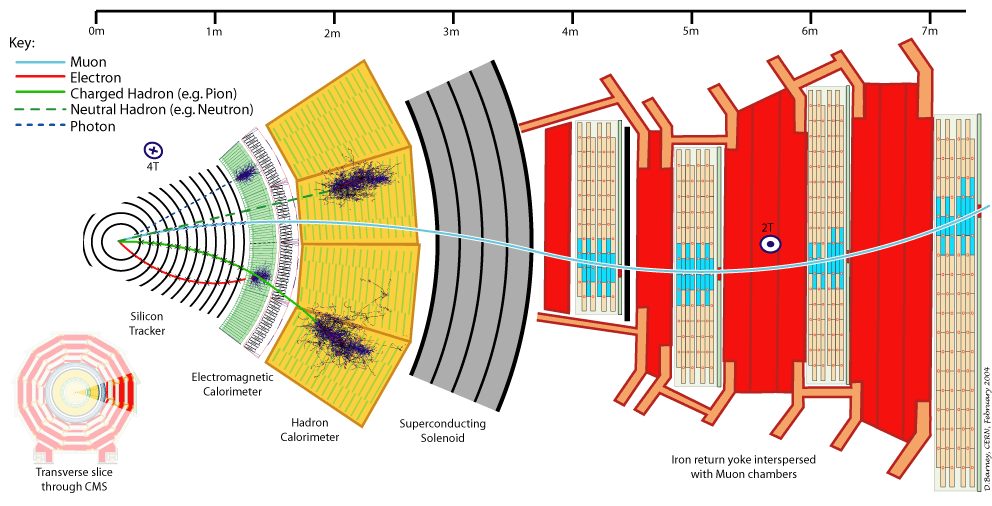
\includegraphics[width=0.9\textwidth]{./Figures/CMS_Slice.jpg}
  \caption{Cross Section of CMS showing the paths of various particle types through different segments of the detector \cite{cmsslice}}
  \label{CMS_SLICE}
\end{figure}

A cross section of CMS is shown in figure \ref{CMS_SLICE}. The coordinate system used by CMS takes the origin at the collision point. The z-axis points along the beam direction and defines the azimuthal angle, $\phi$. Instead of the polar angle, $\theta$, the psuedorapidity, $\eta=-ln(tan(\theta/2))$, is used as $\Delta \eta$ between two particles is relativistically invariant. The eta "coverage" of CMS is $|\eta|<5$. Transverse energies and momenta ($E_T $ and $p_T$)  are defined perpendicular to the beam \cite{cmsiop}. The different detector components shown in figure \ref{CMS_SLICE} will now be described in detail.
\begin{description}
\item[Silicon Tracker]The job of the tracker is to measure the momentum of charged particles from their path through a magnetic field. The CMS tracker achieves $10\mu m$ accuracy with coverage for $|\eta|<2.5$.
\item[Electromagnetic Calorimeter (ECAL)] The ECAL measures the energy of incident photons and electrons. The ECAL is made of 61,200 $PbWO_4$ crystals and provides coverage for $|\eta|<3.0$\cite{ecal}.
 \item[Hadronic Calorimeter (HCAL)] The HCAL is made from alternating brass and scintilator layers with a coverage of $|\eta|<3.0$\cite{hcal}. The coverage is extended to  $|\eta|<5.0$ by an iron/quartz forward calorimeter\cite{hfhcal}. 
 \item[Muon Chambers]The muons are not stopped by any of the calorimeters and therefore require a separate detector with coverage $|\eta| < 2.4$. The muon chambers are interspersed with the magnet return yoke. The high magnetic field allows for accurate momentum measurement\cite{muons}.
\end{description} 
% % Chapter Template

\chapter{Signal Region Optimisation} % Main chapter title

\label{Chapter3} % Change X to a consecutive number; for referencing this chapter elsewhere, use \ref{ChapterX}

\lhead{Chapter 3. \emph{Signal Region Optimisation}} % Change X to a consecutive number; this is for the header on each page - perhaps a shortened title

%----------------------------------------------------------------------------------------
%	SECTION 1
%----------------------------------------------------------------------------------------
%\section{Strategy in Run 1}

In order to maximise sensitivity to a wide range of signal models 
the final analysis bins must be carefully chosen. 
In Run 1 a flat $\alphat > 0.55$ requirement was used. However, 
while the \alphat variable is highly adept at removing the
QCD multijet background it may not be optimal for distinguishing 
signal from the remaining background. Additionally, each bin can have
only one \alphat (and therefore \mht) threshold and no advantage 
may be taken of the shape. Finally, each jet category has the same 
\alphat threshold per \scalht bin. Even with genuine \met  higher jet multiplicities lead to 
lower \alphat values and so more flexibility is desirable. 
In this section when the \scalht bin for each particular jet and btag 
category is considered this will be denoted as \scalhtcat.


\section{Strategy for Run 2}

Taking into account trigger requirements and QCD backgrounds the \alphat thresholds are minimised in each bin. These may be revised after studies with data. Sensitivity is optimised
by using a new discriminating variable such as \mht to conduct a shape analysis in each \scalhtcat bin. 
%To remain data driven a requirement is made on the number of expected control counts for the highest new variable threshold. 
In each \scalhtcat bin the normalisation and systematics are set by the control samples
and closure tests described in Section~\ref{sec:bkgd-est}. The scale of the event is
thus fully controlled in data. Investigations are underway for how the shapes 
and systematics can be found using the shape in the control regions. Given the low
counts in the tails some kind of fit and extrapolation would be required. To minimise the extrapolation a conservative requirement of 10 expected control events is made on the highest new variable threshold. 
%Alternatively the systematics may be estimated entirely from MC by varying the main 
%sources of systematic uncertainty and finding the effect on the shape.

\section{Likelihood Model}

The likelihood model used previously is described in detail in \cite{search}. 
In each \scalhtcat bin there is an uncorrelated (log normal) nuisance per transfer factor for the control prediction. The shape analysis adds an additional dimension.
There will be an additional nuisance for each systematic shape uncertainty.

All results shown are calculated using asymptotic formulae. 
A study was carried out into the reliability of this estimation and the results shown in \ref{asympToys}. 
As seen the differences between CLs toy and the asymptotic formulae are below 10\%.

\begin{figure}
  \centering
  %  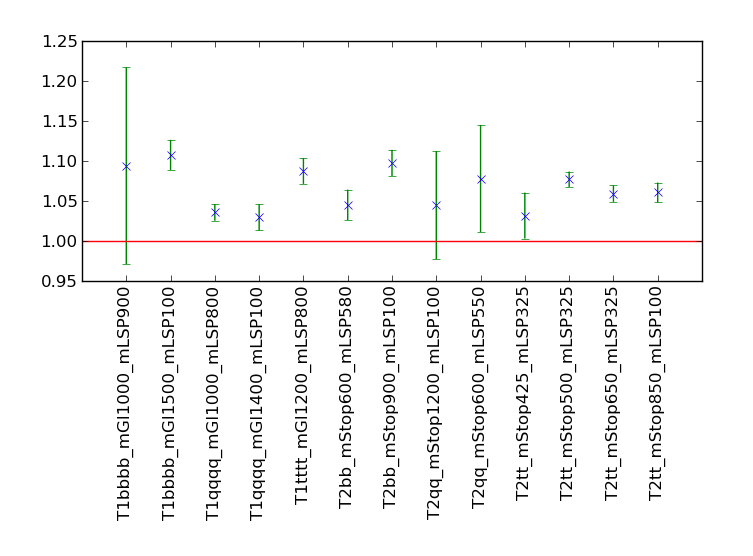
\includegraphics{Figures/asympToys.png}
     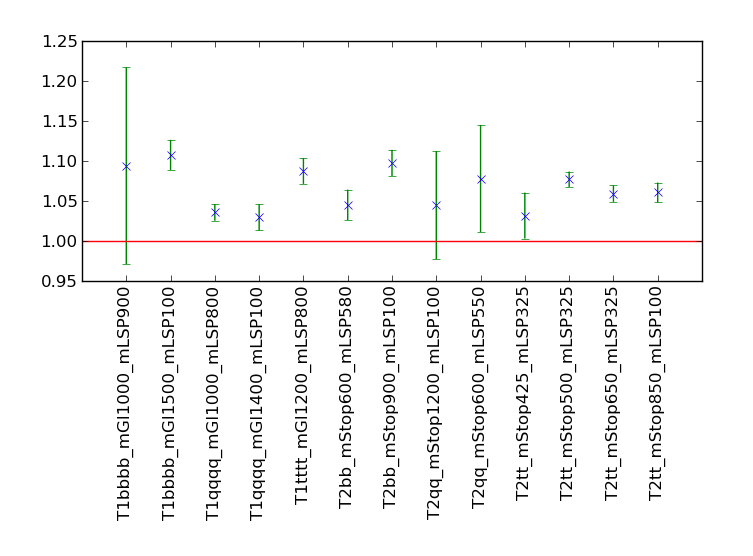
\includegraphics[width=0.7\textwidth]{Figures/asympToys.png}
  \caption{Comparison between asymptotic and toy MC limits}
  \label{fig:asympToys}
\end{figure}

\section{Results}

In order to compare strategies in the absence of data the shape systematics must be estimated. A template for the plus one sigma systematic is found by multiplying each shape by an expontential such that 
the difference from the nominal is set to X\% in the final bin 
and the normalisation is unchanged. The down one sigma templates are found by 
dividing by the same exponential and normalising. Results below are shown
for 10/fb. Luminosity scenarios of 1/fb, 3/fb and 10/fb are under consideration.
To be conservative systematics derived in Run 1 are utilised for the normalisation.

The variables considered were \alphat, \mht,$\mht/\scalht$, $\mht/\sqrt{\scalht}$ and 
$M_eff$ ($\mht+\scalht$). The significances for a shape systematic 
scenario of X=50\% and 10/fb are shown in Figure~\ref{fig:signif}. 

\begin{figure}
\centering
    \includegraphics[width=0.6\textwidth]{Figures/signif}
  \caption{The \alphat distribution shown for a particular search region. The QCD background is completely removed by an \alphat cut at 0.55 while processes with true \met remain.}
  \label{fig:signif}
\end{figure}

As can be seen the \mht variable is consistently near or at the highest 
significance. This can be expected as both compressed and uncompressed models can be expected 
to have significant \mht even though the \scalht scales are very different. Variables optimised
for compressed models (e.g. $\mht/\scalht$) and large mass splittings (e.g. $M_eff$) cannot perform consistently across a range of topologies.

To evaluate the effect on performance of using a shape analysis compared to the
Run 1 strategy several different shape systematics are compared. The results 
are shown in Table~\ref{table:syst} for $X = 0,50,100\%$. Even for the conservative
$X=100\%$, significant gains over the previous strategy can be seen. Comparing
$X=50,100\%$ to $X=0\%$ emphasises the importance of correctly evaluating the uncertainties on the shape.

\begin{table}[!h]
  \label{table:syst}
  \caption{Summary of the siginificances found for shape analysis compared
    with the Run 1 strategy. Even with 100\% error in the final bin
  the shape analysis performs significantly better than before.}
  \centering
  \footnotesize
  \begin{tabular}{ l | l | l | l | l | l | l }
    Model & Mass/GeV & LSP Mass/GeV & Run 1 & Shape (X=0) & Shape (X=50) & Shape (X=100) \\ \hline
    T2tt & 650 & 325      & 1.09& 1.83& 1.38& 1.27\\ 
    T2tt & 500 & 325      & 0.60& 1.93& 1.42& 1.33\\ 
    T2tt & 425 & 325      & 1.11& 2.25& 1.79& 1.65\\ 
    %T2qq & 600 & 550     & 4.38& 8.98& 6.01& 5.19\\ 
    T2qq & 1200 & 100      & 1.10& 3.17& 2.37& 2.14\\
    T2bb & 900 & 100      & 1.54& 1.85& 1.59& 1.48\\ 
    T2bb & 600 & 580      & 0.35& 0.81& 0.60& 0.53\\ 
    T1tttt & 1500 & 100    & 1.04& 3.10& 2.65& 2.58\\
    T1tttt & 1200 & 800    & 0.77& 1.63& 1.15& 1.09\\
    T1qqqq & 1400 & 100    & 0.86& 4.71& 3.17& 2.50\\
    T1qqqq & 1000 & 800    & 2.45& 4.53& 2.90& 2.40\\
    T1bbbb & 1500 & 100    & 2.41& 6.93& 5.82& 5.61\\
    T1bbbb & 1000 & 900    & 3.61& 7.12& 5.61& 5.29\\
  \end{tabular}
\end{table}

% \subsection{Automated Binning}
%
% To determine the binning in the NV an automated procedure is used. Initially this is run for each signal model separately and works as follows. 
% \begin{enumerate}
% \item To ensure the analysis remains data driven the NV threshold is chosen such the number of events in the control samples (not split in btags) for the relevant backgrounds is sufficient to carry out closure tests. This threshold is then used as an upper bound for the NV binning ($NV_{closure}$). 
%   \item This the systematic error is taken from closure tests. This will be \scalhtcat dependant for the case of correlated NV bins or also NV dependant if the NV bins are decorrelated.  	
%   \item The signal and background counts integrated from each NV threshold to $\infty$ are found.
%   \item The systematic error is added in quadrature to the statistical error determined from the transfer factor from the control region to the signal region.
%   \item The significance is the found for every possible NV cut value using the asymptotic formula considering data counts given by background plus signal contribution and the background only prediction with the uncertainty determined above. This is truncated at $NV_{closure}$.
%   \item The significance is then smoothed to remove fluctuations and the maximum is assigned as the highest lower bin threshold.
%   \item The procedure is repeated integrating up to the lower bin threshold found in the previous step. A minimum bin width is enforced to minimise bin migration.
%   \item The procedure stops when the significance is below a predetermined threshold.
% \end{enumerate}
% \begin{table}[h!]
%   \caption{\alphat and (effective) \mht thresholds per \scalht bin.\label{tab:alphat-thresholds}. For the $>$800 bin there is a direct \mht rather than \alphat requirement}
%   \centering
%   \footnotesize
%   \begin{tabular}{ lccccccc }
%     \hline
%     \hline
%     \scalht      & 200--250   & 250--300   & 300--350  & 350--400  & 400--800 \\ & $>$800       \\
%     \hline                                                                     
%     \alphat      & 0.65       & 0.60       & 0.55      & 0.53      & 0.52     \\  & 0         \\
%     "Min \mht"   & $\sim$128  & $\sim$138  & $\sim$125 & $\sim$133 & $\sim$137 \\  & 130 \\
%     \hline
%     \hline
%   \end{tabular}
% \end{table}
%
% To ensure the same bins are used for all signal models a representative selection of models are used to determine the optimal binning for each \scalhtcat bin. The model with the highest exclusion in each bin then determines the binning. This is done for every \scalhtcat bin and a standard binning is found for all models.
% \subsection{Strategies}
%
% There are several possible strategies for binning and utilising the data in each \scalhtcat bin. The most similar approach to the previous strategy is simply to choose NV thresholds (per \scalht) which map closely to the \alphat requirements used in Run 1 (S0). Following from this is to run the optimisation procedure described below and use the last NV threshold in each \scalhtcat bin (S1). In these cases systematics are detemined via the closure tests in exactly the same way as for Run 1.
%
% The last two strategies take advantage of the full range of the NV. The more conservative approach is to determine uncorrelated systematics in the NV dimension via closure tests and use these to determine bin thresholds per NV value. These systematics are used in the optimisation and the likelihood is fully binned with uncorrelated systematics along the NV dimension (S2). This has the advantage of remaining purely data driven. Finally, a shape analysis can be used. In this case there is no need for optimisation. The normalisation systematic is the same as for S0 and S1 (fully determined by data) but templates generated using Monte Carlo in the signal region for each dominant systematic source are used as the shape systematics for each background source along the NV dimension.

% % Chapter 4

\chapter{SuperSymmetry} % 

\label{Chapter4} % For referencing the chapter elsewhere, use \ref{Chapter1} 

\lhead{Chapter 4. \emph{SUSY}} % This is for the header on each page - perhaps a shortened title

%----------------------------------------------------------------------------------------

\section{Supersymmetry}

Supersymmetry is an extension of the symmetries of the standard model by anticommuting operators which generate transformations from a fermion to boson state and vice versa to form supermultiplets \cite{susyintro}. It is for the heavy superpartners of SM particles that experiments such as the LHC search. The theoretical motivations for SUSY lies in the effect on the ultra-violet energy region. For example, unlike the SM, the couplings to the Higgs need not be fine-tuned to remove divergences. The mass found for the Higgs, at around 126 GeV, agrees well with phenomenological models of SUSY with superpartners around the TeV scale (and so potentially observable)\cite{susyhiggs}. 
\subsection{SUSY as a replacement for the SM}
The SM has shown remarkable agreement with experiment. In the few cases in which there is tension, such as the anomalous g-2 measurement \cite{gm2}, SUSY is only able to accommodate rather than directly explain the anomalies. One exception to this is dark matter. This is a Weakly Interacting Massive Particle (WIMP) which appears to account for various astrophysical observations of gravitational excesses compared to the observed baryonic matter\cite{dm}. The MSSM imposes R-Parity which is defined in equation \ref{Rparity}. 
\begin{equation}
\label{Rparity}
P_R=(-1)^{2s+3B+L}
\end{equation}
Where s is spin, B is baryon number and L is lepton number. These quantities have been shown to be conserved to a very high accuracy. As SUSY particles have $P_R=-1$ while SM particles have $P_R=1$ R-Parity conservation restricts the decay and production modes of SUSY particles\cite{susywimp}. Crucially for dark matter, the Lightest Supersymmetric Particle (LSP) is prevented from decaying and may be a WIMP. Ensuring the LSP is a dark matter candidate provides stringent theoretical limits on the MSSM.

\subsection{SUSY Searches}
As the LHC is a hadron collider the strong force modes, gluino and squark pair production, will dominate. Depending on the MSSM model the decay of these sparticles produces different signatures such as leptons or high jet multiplicity. Different search strategies are thus essential. As the decay chain must end with the LSP a key signature for all of these searches is missing energy. The $\alpha_T$ analysis relies on an all-hadronic final state with multiple jets along with large missing energy production. 

\section{$\alpha_T$}
Large SM backgrounds are caused by vector boson decays to neutrinos and mismeasured QCD. Calculating $\cancel{\it{E}}_{T}$ requires precise information from each of the calorimeters, tracking and muon subdetectors. This can easily lead to "fake" missing energy in the final state from mismeasured QCD jets\cite{randall}. Such a source can be particularly expected in the uncertain environment just after turn on.  The $\alpha_T$ variable has been designed explicitly to remove this source of background and is defined in equation \ref{alph}.
\begin{equation}
\label{alph}
\alpha_T=\frac{1}{2}\frac{1-(\Delta H_T/H_T)}{\sqrt{1-(\cancel{H_T}/H_T)^2}}
\end{equation}
This is defined for n-jets by creating a pseudo di-jet system which minimises the difference in energy between the two pseudo jets ($\Delta H_T$). The total transverse energy is defined as $H_T=\sum_{i=1}^nE_t^{j_i}$ and $\cancel{H_T}=|{\sum_{i=1}^n p_T^{j_i}}|$. Unlike SUSY, $\Delta H_T$ and $\cancel{H_T}$ are highly correlated for energy mismeasurement and neutrinos from heavy-flavour quark decays. This means that QCD backgrounds should have $\alpha_T<0.5$ whereas for SUSY it is unrestricted. In the latest $\alpha_T$ search for $8 TeV$ the cut is on $\alpha_T<0.55$ which is sufficient to make such backgrounds negligible. A sample distribution of $\alpha_T$ from this search is shown in figure \ref{alphdis} \cite{CMSAT8}.
\begin{figure}
\centering
    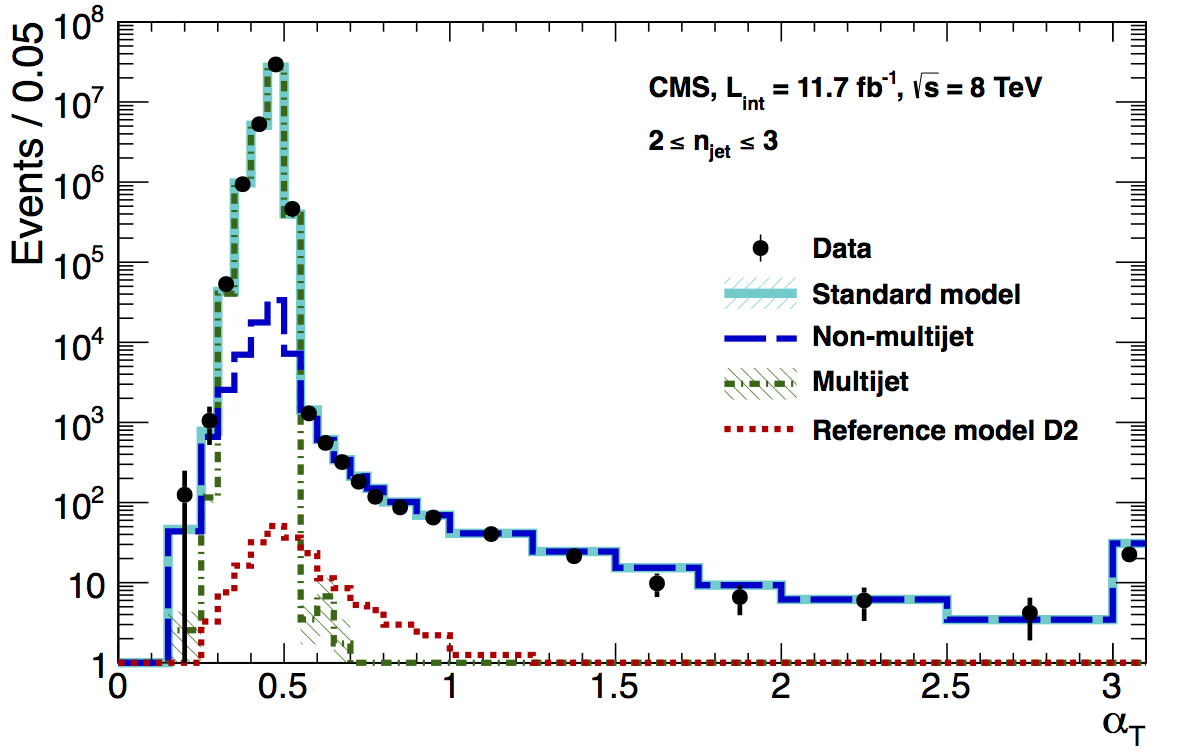
\includegraphics[width=0.8\textwidth]{Figures/sample_aT.jpg}
  \caption{$\alpha_T$ distribution shown for a particular search region. The contribution from a SUSY reference model shows events above 0.55.}
  \label{alphdis}
\end{figure}

\subsection{Background Reduction}
The remaining background from electroweak processes must be estimated. This includes missing energy from $Z\rightarrow\nu\nu$ and $W\rightarrow\nu\tau$ where the $\tau$ decays hadronically. To minimise dependence on Monte Carlo a data driven approach is taken. The number of events in control regions with low signal contamination is measured. Then the effect in the signal region is predicted using equation\ref{control}. This is cross checked using closure tests.
\begin{equation}
\label{control}
N_{pred}^{signal}=\frac{N_{MC}^{signal}}{N_{MC}^{control}}\times N^{control}_{obs}
\end{equation} 
\subsection{Signal Regions}
Signal regions are defined to emphasise sensitivity to different SUSY models\cite{CMSAT8}. They are split into different energy regions as well as jet multiplicity and number of b-jets to increase statistical significance. The b-tagging is important as, due to the inverted mass hierarchy, $\tilde{b}$ and $\tilde{t}$ are the lightest squarks and will decay via b-jets.
\subsection{Interpretation}
Finally the data from CMS must be interpreted. This is done using simplified models which have only one production and decay mode and are a measure of the reach of a search in parameter space. Two sample simplified model decays from the latest 8 TeV $\alpha_T$ analysis involving decays to quarks are shown in figure \ref{simp}. Each simplified model is suited to a different signal bin. The model predictions for different parent and LSP masses are then confronted with the background estimation along with the data to make mass exclusion planes. These are shown in figure \ref{simp2} for the latest search.
\begin{figure}
\hfill
\subfigure[Squark Production (T1)]{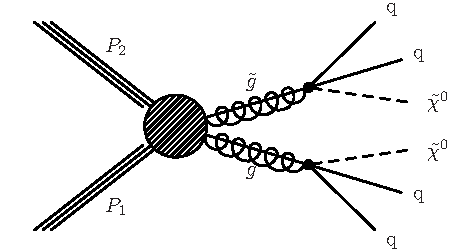
\includegraphics[width=5cm]{Figures/T1}}
\hfill
\subfigure[Gluino Production (T2)]{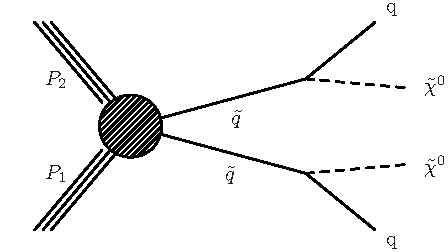
\includegraphics[width=5cm]{Figures/T2}}
\hfill
\caption{Two typical simplified models involving gluino and squark decays to quarks}
\label{simp}
\end{figure}
\begin{figure}
\hfill
\subfigure[T1 Exclusion]{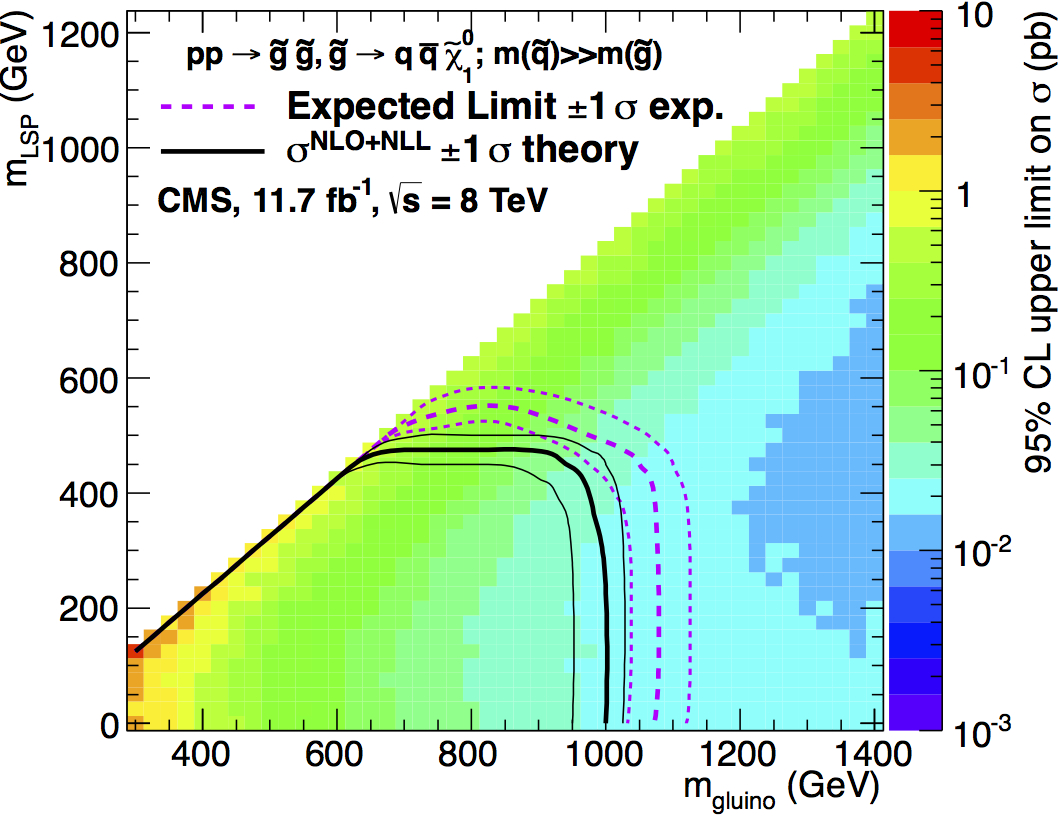
\includegraphics[width=7cm]{Figures/T1plot}}
\hfill
\subfigure[T2 Exclusion]{\includegraphics[width=7cm]{Figures/T2plot}}
\hfill
\caption{Exclusion planes for two simplified models}
\label{simp2}
\end{figure}


 
% Chapter Template

\chapter{Conclusions} % Main chapter title

\label{Chapter6} % Change X to a consecutive number; for referencing this chapter elsewhere, use \ref{ChapterX}

\lhead{Chapter 6. \emph{Conclusions}} % Change X to a consecutive number; this is for the header on each page - perhaps a shortened title

%----------------------------------------------------------------------------------------
%	SECTION 1
%----------------------------------------------------------------------------------------

\section{Conclusions}
This report has covered the general motivations of SUSY. One particular search, $\alpha_T$ has been described and its effectiveness after turn-on has been explained. The results from searches such as $\alpha_T$ are presented using simplified models allowing their reach in parameter space to be quantified. While this has deeply constrained new theories of physics the central motivation for low mass SUSY -- to stabilise the Higgs mass naturally -- remains. The LHC upgrade will provide significantly increased energies and luminosities. The effect this will have on SUSY production cross sections is shown in figure \ref{snow}\cite{ProjectedCx}. As can be seen the quantity of predicted SUSY events will be significantly increased. If low mass SUSY is physical then the LHC upgrade and $\alpha_T$ will provide an excellent opportunity for discovery. 
\begin{figure}
\centering
    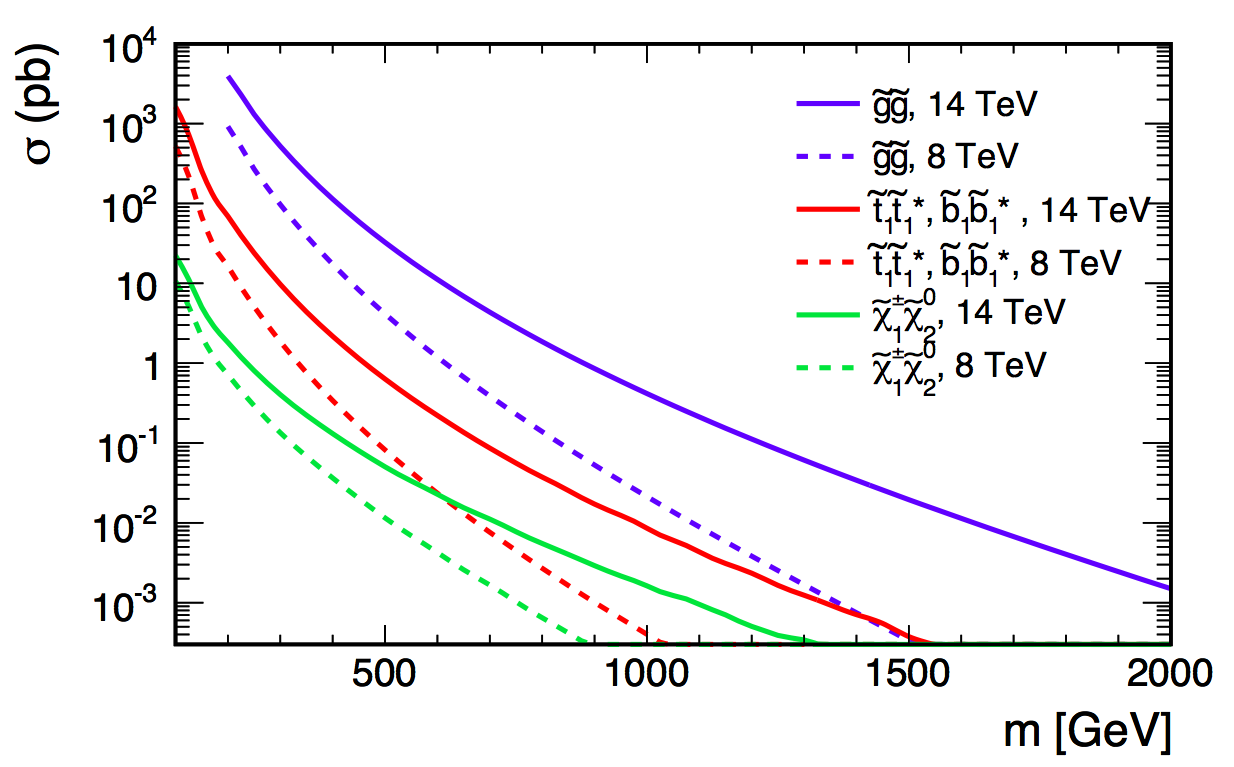
\includegraphics[width=0.8\textwidth]{Figures/snowmass.png}
  \caption{SUSY production cross sections at 14 TeV compared with 8TeV}
  \label{snow}
\end{figure}


 
% Chapter Template

\chapter{Pile Up Studies} % Main chapter title

\label{Chapter 6} % Change X to a consecutive number; for referencing this chapter elsewhere, use \ref{ChapterX}

\lhead{Chapter 6 \emph{pileup Studies}} % Change X to a consecutive number; this is for the header on each page - perhaps a shortened title

%----------------------------------------------------------------------------------------
%	SECTION 1
%----------------------------------------------------------------------------------------

\section{Jet}
\subsection{Efficiencies}
In order to test the jet finding algorithm the first study that must be undertaken is into the matching efficiency of the L1 jets to generator level quantities (gen jets). A simulated sample of $t\bar{t}$ pairs was used\footnote{In this report all simulated samples used have conditions of $13TeV$ collisions with bunch spacing $50ns$. The pileup is gaussian distributed around $40$ interactions per bunch crossing}. The gen jets are made by running the anti-kt algorithm with radius parameter $R=0.4$ on generator level quantities. The gen jet is said to be matched if it is within ${\Delta R}^2<33$ of a L1 jet (the greatest extent of the L1 jet). The matching efficiency for alljets and the fourth jet is shown in figure \ref{match}. It can be seen that the efficiency after pileup subtraction/seed drops at low $p_T$ this motivates a cut at $30GeV$ for calculation of energy sums. Inefficiencies at high $p_T$ are caused by the `chain veto', however, the jet algorithm guarantees there is always a comparable or higher jet in the event in such cases. The performance compared to GCT is seen to be greatly improved.  
\begin{figure}
\hfill
\subfigure[All jets\label{fig:label:alljet}]{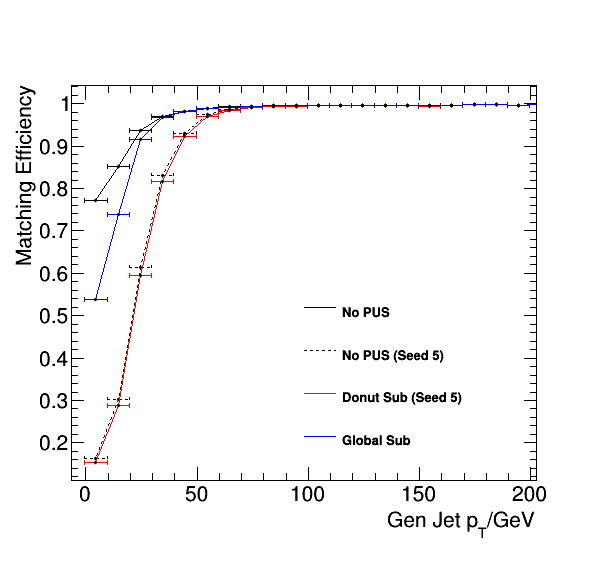
\includegraphics[width=6.9cm]{Figures/alljet}}
\hfill
\subfigure[4th jet\label{fig:label:jet4}]{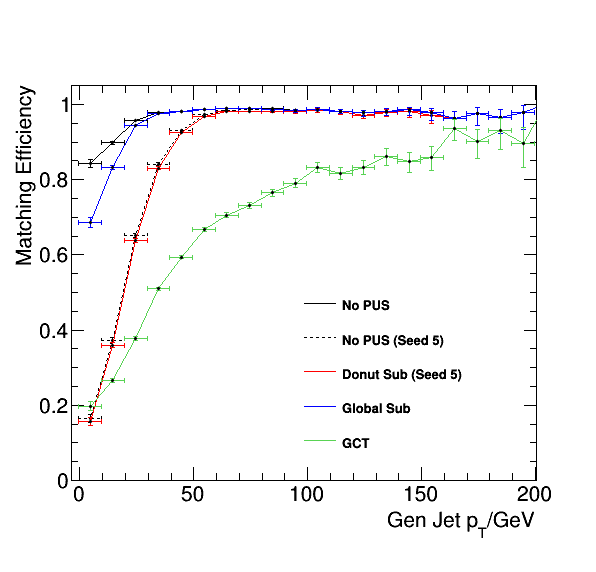
\includegraphics[width=7cm]{Figures/jet4}}
\hfill
\caption{Matching efficiencies for jets showing effect of seed and pileup subtraction at low energies. In \ref{fig:label:jet4} a comparison with the GCT is shown.}
\label{match}
\end{figure}
\subsection{Calibration}
The energy of the L1 jets is calibrated using generator level quantities. The scheme for calibration is outlined in \cite{l1jet_calibration}. The calibration is carried out in bins of $\eta$ to account for the difference in performance of the detector. Using a QCD sample, the response (defined as $p^{L1}_{T}/p^{gen}_{T}$) and $p^{L1}_{T}$ are plotted against $p^{gen}_{T}$ and fitted. The fits are then plotted against each other and the result itself fitted giving calibration factors as a function of $p^{L1}_{T}$.  Where the matching efficiency is low it is not possible to fit and so the calibration has a lower bound on $p_T$. This was found to occur at $30GeV$. An upper bound is defined by where the fits become statistically limited. This was found to occur at $300GeV$. If the fit is well defined the calibration factor should flatten with increasing $p_T$ and so higher $p_T$ jets may still be calibrated by continuing the fit. The calibration factors change depending on the pileup subtraction regime. In figure \ref{calib} the effect of the calibration is shown.   

\begin{figure}
\centering
    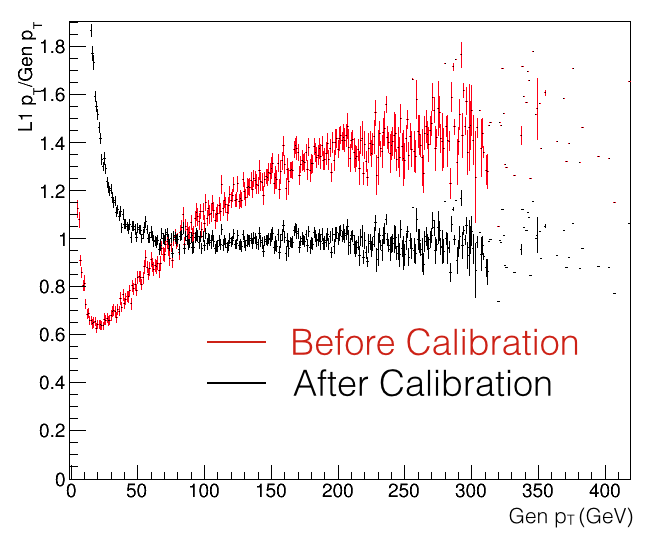
\includegraphics[width=7cm]{./Figures/calibration}
  \caption{Effect of calibration on donut subtracted jets. At the limit of calibration ($30GeV$) the difference for the calibrated sample is around $10\%$.}
  \label{calib}
\end{figure}
\section{Pileup Subtraction Testing}

\subsection{Resolution dependence on number of interactions}
In this section plots are shown for the highest $|\eta|$ bin as the detector performance is expected to worsen with larger $|\eta|$ and so pileup subtraction will have the largest effect. The first test of any pileup subtraction scheme is the effect on the resolution. In an ideal post pileup subtraction scenario this will be flat as a function of the number of interactions. In figure \ref{fig:label:resolution1} this is plotted for a particular $p^{gen}_T$ and $\eta$ bin. It can be seen that the response flattens for both pileup subtraction regimes. This is summarised in \ref{fig:label:resolution2} where the gradient from the fit to the resolution plot is shown to reduce after pileup subtraction for a range of $p^{gen}_T$ bins.  
\begin{figure}
\hfill
\subfigure[\label{fig:label:resolution1}]{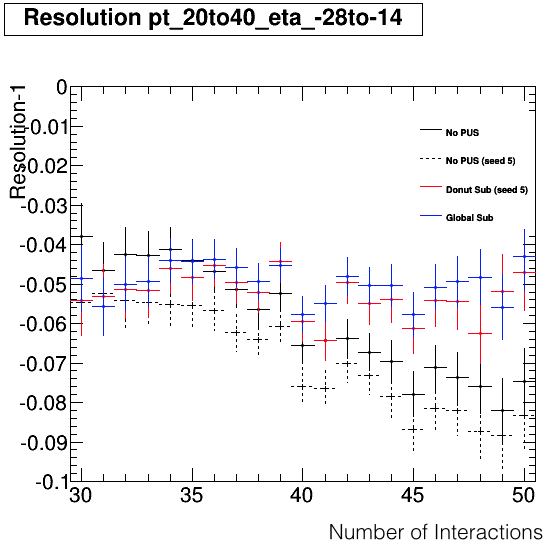
\includegraphics[width=6.8cm]{Figures/resolution}}
\hfill
\subfigure[\label{fig:label:resolution2}]{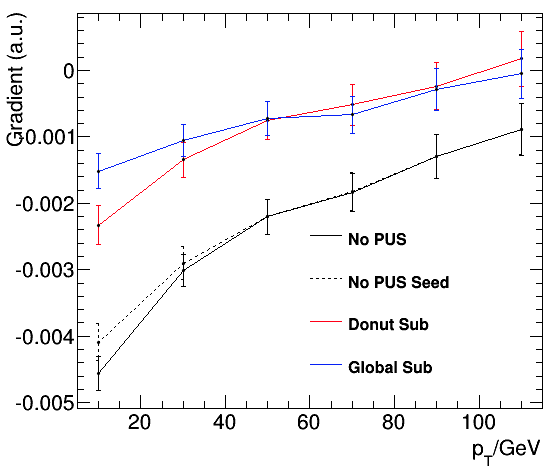
\includegraphics[width=7.1cm]{Figures/p1eta_14to28_calib_fits}}
\caption{In \ref{fig:label:resolution1} response versus number of interactions is shown for a particular eta bin showing the response flattens after pileup subtraction. In \ref{fig:label:resolution2} the fit gradient for different $p_{T}$ bins is shown.}
\label{fig:label:resolution}
\end{figure}
\subsection{Rates}
The rate is defined as the proportion of jets for background passing a particular $p_{T}$ cut. For the efficiency a cut is made on the gen jets ($50GeV$). The proportion of these events with a corresponding matched L1 jet over a threshold then defines the efficiency at that threshold.  For the trigger the key test is to see that the efficiency for signal may be maintained while reducing the background rate. For the background a pure pileup sample was used while the $t\bar{t}$ samples was used for signal. In figure \ref{fig:label:ratejet1} the rate is shown for the leading jet. The performance compared to the GCT is shown to be improved. The seed cut appears to have the largest effect in reducing the rate as global is shown to be comparable to no pileup subtraction. Figure \ref{fig:label:ratenvtx} shows the evolution of the rate with the number of interactions. GCT shows the largest dependence, as expected, while for stage 2 pileup subtraction is shown to flatten this dependence. Applying donut subtraction appears to increase the rate compared to applying a seed alone. This may be due to contamination causing over subtraction. The calibration will then bring the energy above the seed. Finally, in figure \ref{fig:label:rateeff} the seed is shown to be comparable to global alone while applying donut subtraction worsens the performance. This may be due to over-subtraction of jets due to contamination for nearby jets in the donut ring.
\begin{figure}
\hfill
\subfigure[Rate Jet 1\label{fig:label:ratejet1}]{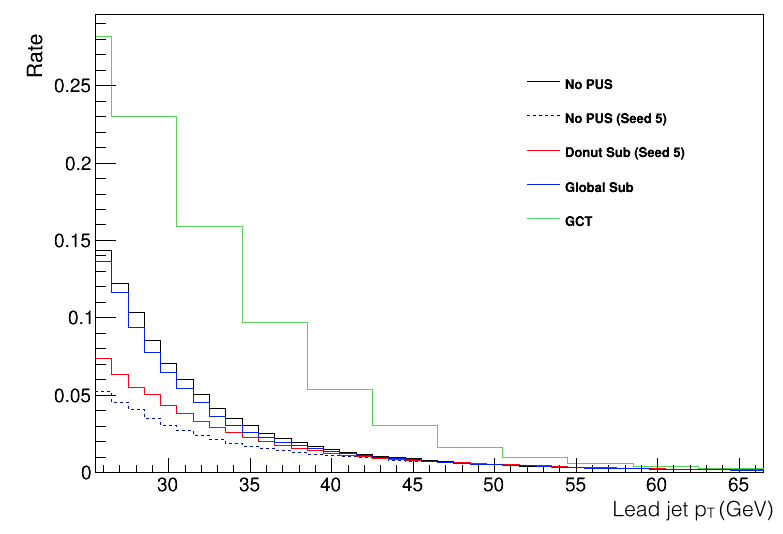
\includegraphics[width=7cm]{Figures/rate_jet1}}
\hfill
\subfigure[Rate Jet 1\label{fig:label:ratenvtx}]{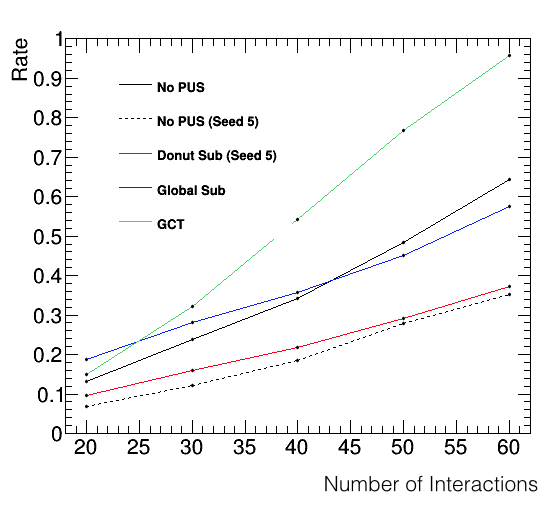
\includegraphics[width=7cm]{Figures/neutrinonvtx_jet1}}
\caption{The dependence of the rates for the lead jet with $p_T > 30 GeV$ on the number of interactions is shown in figure \ref{fig:label:ratenvtx} while\ref{fig:label:ratejet1} shows improved rate for stage 2 compared to GCT and for pileup subtraction.}
\label{fig:label:rates}
\end{figure}
\begin{figure}
\centering
    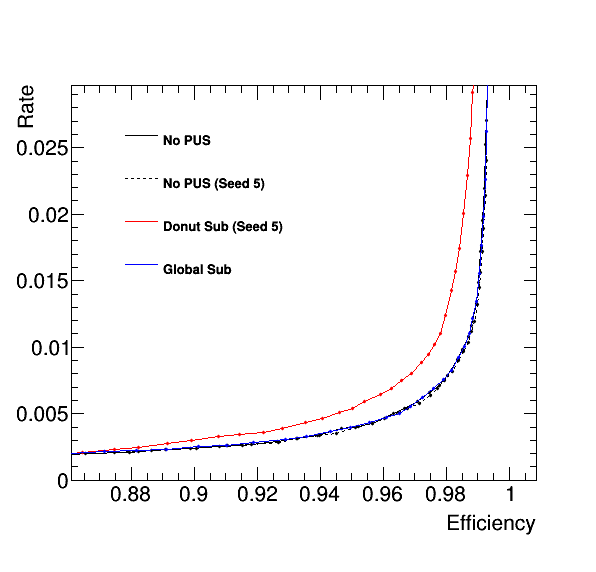
\includegraphics[width=10cm]{./Figures/jet1RateEff}
  \caption{Rate versus efficiency for lead jet. Performance is consistent except for donut which appears to excessively reduce efficiency}
  \label{fig:label:rateeff}
\end{figure}
\subsection{Turn On Plots}
To benchmark the performance of the L1 jets their $p_T$ must be compared with matched generator level quantities. To do this the generator level quantity is plotted with a cut on the matched L1 quantity (the turn on). This is shown for two representative examples in figure \ref{turnon}. As can be seen the turn on for the GCT is less sharp than that for the stage 2 quantities. Donut subtraction is seen to be inefficient at higher $p_T$ values. This suggests contamination for nearby jets or fluctuations in the donut ring causes such jets to have lower $p_T$.
\begin{figure}
\centering
    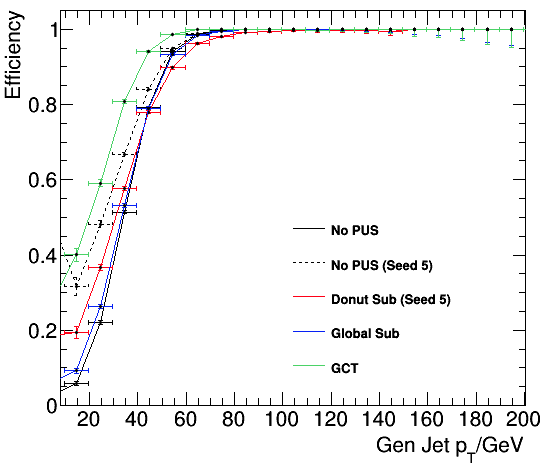
\includegraphics[width=0.8\textwidth]{Figures/jet4_40}
  \caption{Turn on curve for the 4th jet at 40 GeV showing comparable behaviour for the stage 2 quantities and a shallower turn on for GCT.}
  \label{turnon}
\end{figure}
\subsection{Energy Sums}
Lastly the energy sums which are used to make triggers based $H_T$ and $\cancel{H_T}$ were investigated. To nullify the problem of the lower calibration limit, only jets above this are included in the sums. Pileup is expected to be approximately uniform and so it should not affect the missing energy in the event. The result for $H_T$ and $\cancel{H_T}$ for a ttbar sample are shown in figure \ref{fig:label:sums}. Pileup subtraction improves the agreement as compared to gen.  The $H_T$ shows especially good agreement with gen for the case of a seed as compared to global. This is due to the under-subtraction bias of the global rho method. The $\cancel{H_T}$ shows similar levels of agreement for all cases as expected. 
\begin{figure}
\hfill
\subfigure[$H_T$\label{fig:label:ht}]{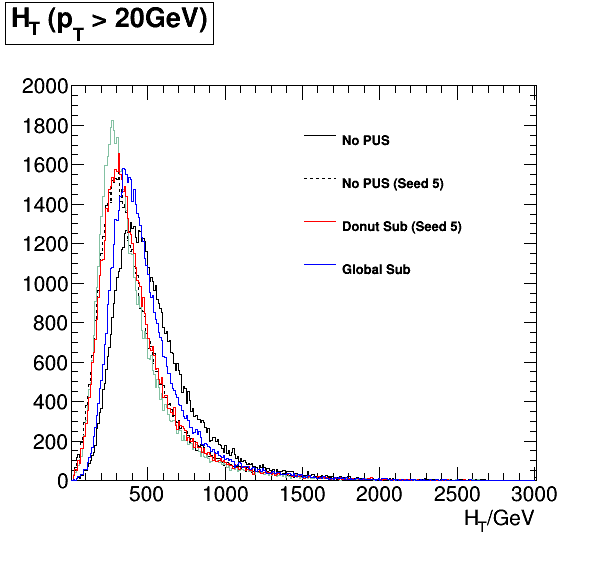
\includegraphics[width=7cm]{Figures/ht_ttbar}}
\hfill
\subfigure[$\cancel{H_T}$\label{fig:label:mht}]{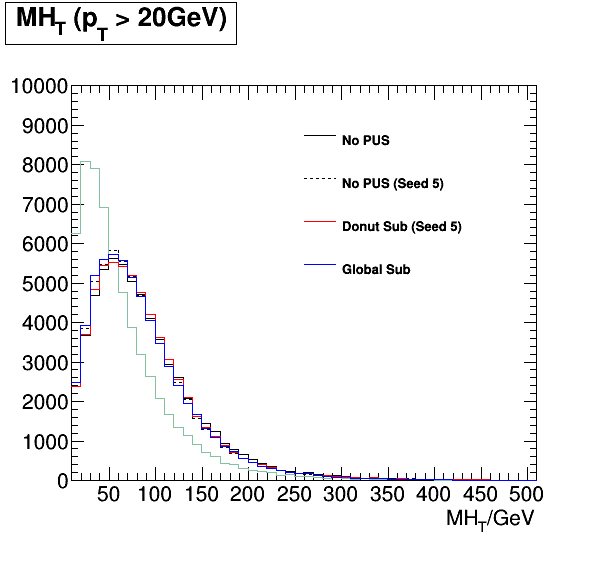
\includegraphics[width=7cm]{Figures/mht_ttbar}}
\caption{In figure \ref{fig:label:ht} the total energy shows good agreement with the generator level quantity. This is improved by requiring a seed threshold. In figure \ref{fig:label:mht} similar agreement is shown for all cases}
\label{fig:label:sums}
\end{figure}
\section{Conclusions}
The jet algorithm has been shown to function well, giving very compatible results with the offline anti-kT algorithm and maintaining a high matching efficiency to generator level quantities. The pileup subtraction studies have shown that pileup subtraction is required for run 2. While both global and donut subtraction have been shown to flatten the response (\ref{fig:label:resolution} each has weaknesses that must be addressed. Figure \ref{fig:label:rateeff} shows that applying a seed threshold is comparable to global subtraction at killing rate while maintaining efficiency. Donut subtraction is shown to perform less well than applying the seed threshold alone. This is due to the susceptibility of donut subtraction to fluctuations and contamination. Further studies are underway to increase the sampling area for donut subtraction to reduce this issue. Figure \ref{fig:label:sums} shows global $\rho$ under-performing for the $H_T$. This is due to the under-subtraction bias leading to more energy being left in the event. This may be correcting by applying a seed threshold as for donut but calculating $\rho$ using all jets. 

Further studies are currently underway to utilise the $\eta$ dependence of the pileup.  The seed threshold applied may be altered depending on the location of the tower to further reduce rate in areas of high pileup while maintaining efficiency in low pileup regions. Improving calibrations such that lower energy jets may be utilised ( the current limit is 20GeV) is also key. Finally, increasing the sample size to use $3\times3$ towers for the seed should improve discrimination between pileup and boosted jets. 

    
 
% % Chapter Template

\chapter{Jets and PU at stage 2} % Main chapter title

\label{Chapter 5} % Change X to a consecutive number; for referencing this chapter elsewhere, use \ref{ChapterX}

\lhead{Chapter 5. \emph{Conclusions}} % Change X to a consecutive number; this is for the header on each page - perhaps a shortened title

%----------------------------------------------------------------------------------------
%	SECTION 1
%----------------------------------------------------------------------------------------

\section{Jet Algorithm}
\label{algo}
The focus of the results in this report will be on studies for jet definitions and pile-up subtraction algorithms for the stage 2 trigger. At stage 2 the TMT allows the granularity to be significantly increased compared to the legacy system. The cells used to make the jets will reduce from $4\times4$ towers to single towers. Due to the increase in energy to 13TeV the jets will be boosted and therefore smaller in size. To account for this at level one the cone size should be decreased. The algorithm presented here uses a cone size of 9 by 9 compared to 12 by 12 which corresponds to the decrease from R=0.5 to R=0.4 in the jet definition proposed for HLT (CITE??). Jets from the primary vertex are likely to be boosted and thus most of their energy is in the central (seed) tower. The algorithm is thus as follows: each trigger tower in turn is taken as the candidate. The towers in the 4 surrounding rings (or up to the edge in $\eta$) are then compared to the seed tower using the mask shown in figure \ref{mask}. If the comparison is true for any tower then the seed is vetoed and the next tower is checked. The mask is designed to be unambiguous for towers of equal energy. If a seed is not vetoed then a jet is defined at that tower position with $p_t$ given by the total energy of the towers.   
\begin{figure}
\centering
    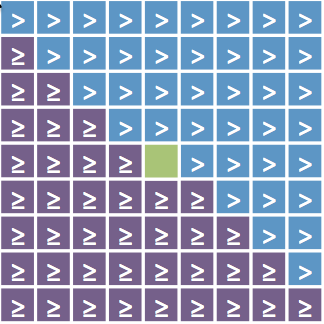
\includegraphics[width=0.5\textwidth]{Figures/mask.png}
  \caption{Nine by nine mask used to define jets}
  \label{mask}
\end{figure}
\newpage
The two main problems with this algorithm are that sufficiently close jets will appear as a single jet and that energy may be lost if a tower that vetoes another is itself vetoed by a tower sufficiently far away not to include the far tower's energy. The first case is common to all jet algorithms with a fixed cone size but as the energy is not lost the single jet or total energy will almost certainly be enough to trigger. Despite this a quality bit adapted from the idea of n-subjetiness \cite{nsub} is under investigation. The lost energy is found to be a small (~0.1\% inefficiency).
%%///ASKJAD%%%
\section{Jet Algorithm}
The focus of the results in this report will be on studies for jet definitions and pile-up subtraction algorithms for the stage 2 trigger. At stage 2 the TMT allows the granularity to be significantly increased compared to the legacy system. The cells used to make the jets will reduce from $4\times4$ towers to single towers. Due to the increase in energy to 13TeV the jets will be boosted and therefore smaller in size. To account for this at level one the cone size should be decreased. The algorithm presented here uses a cone size of 9 by 9 compared to 12 by 12 which corresponds to the decrease from R=0.5 to R=0.4 in the jet definition proposed for HLT (CITE??). Jets from the primary vertex are likely to be boosted and thus most of their energy is in the central (seed) tower. The algorithm is thus as follows: each trigger tower in turn is taken as the candidate. The towers in the 4 surrounding rings (or up to the edge in $\eta$) are then compared to the seed tower using the mask shown in figure \ref{mask}. If the comparison is true for any tower then the seed is vetoed and the next tower is checked. The mask is designed to be unambiguous for highest towers of equal energy. If the seed is not vetoed then a jet is defined at that tower position with $p_t$ given by the total energy of the towers.    
\begin{figure}
\centering
    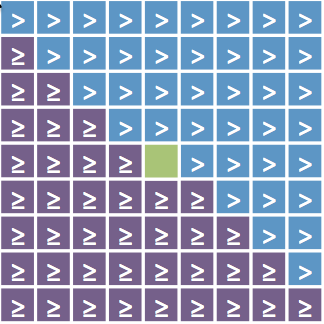
\includegraphics[width=0.5\textwidth]{Figures/mask.png}
  \caption{Nine by nine mask used to define jets}
  \label{mask}
\end{figure}
\newpage
The two main problems with this algorithm are that sufficiently close jets will appear as a single jet and that energy may be lost if a tower that vetoes another is itself vetoed by a tower sufficiently far away not to include the far tower's energy. The first case is common to all jet algorithms with a fixed cone size to avoid duplication of energy but as the energy is not lost the single jet or total energy will almost certainly be enough to trigger. Despite this, a quality bit adapted from the idea of n-subjetiness \cite{nsub} is under investigation this would allow a jet with substructure but with lower energy than the single jet threshold to trigger. The energy lost by a 'chain' veto is an unavoidable inefficiency, however, the effect of this is seen to be small in the matching (~0.1\% inefficiency) (see figure**).

\section{Pile Up Subtraction}
\subsection{Pile Up}
The luminosity of the LHC will be increased in the upgrade to $L = 1\times10^{34} cm^{-2}s^{-1}$. The easiest way to increase luminosity while maintaining stability is to use large, but widely separated, proton bunches \cite{pileup}. However, for the detector this means increased number of primary vertices (pile up) at the collision point. The average number of vertices per bunch crossing is given in equation \ref{pu}.

\begin{equation}
\langle N_p \rangle = \sigma L \tau_b
\label{pu}
\end{equation}

where $\langle N_p \rangle$ is the average number of vertices, $\sigma$ is the cross section and $\tau_b$ is the bunch spacing. At the end of run 1 with $8 TeV$ ($\sigma = 71.5mb$),$\tau_b = 50ns$ and $L = 0.75\times10^{34} cm^{-2}s^{-1}$ gave $\langle N_p \rangle$ = 27. After LS1 the luminosity and $\sigma$ gain (to $76mb$) this will increase to $\langle N_p \rangle$ = 40. 
\subsection{Effect of Pile Up}
The majority of PU events are low energy QCD processes which will appear as randomly distributed energy in the calorimeter region (about 1 GeV per unit area). This PU can have two detrimental effects for the L1 trigger. Firstly, when the PU is evenly distributing the energy of the real jets is slightly increased thus artificially increasing the total transverse energy. The second problem occurs when the PU is randomly clustered - significantly boosting a single jet or forming fake jets. Due to the non perfect response of the detector and profile of the PU these effects may be dependent on $\eta$. In order to trigger only on hard events the effect of the PU must be mitigated (subtracted). In this report two example methods of pileup subtraction (global $\rho$ and donut) will be discussed.
\subsection{Subtraction}

M. Cacciari and G. P. Salam, “Pileup subtraction using jet areas,” Phys.Lett., vol. B659, pp. 119–126, 2008

If the detector response is assumed to be approximately $\eta$ independent then one may use an event based PU subtraction. In the case of global $\rho$ first all the jets are reconstructed using the algorithm in \ref{algo}. The jets are then ranked in order of energy density $\rho$ where for jet i, $\rho^i$ is defined in equation \ref{rho}.
\begin{equation}
\label{rho}
\rho^i = \frac{p^i_{T}}{A_i} 
\end{equation}
where $A_i$ is the area of the jet. The median $\rho$ ($\rho^m$) of the jets is then taken as the estimator of the PU energy density in the event. All jets are in the event then reduced in energy by $\rho^m \times A^i$ and those with $p_{T}^i < \rho^m \times A_i$ taken to be PU and removed. The correlation of this parameter with the number of vertices is shown in figure **. This method has the advantage of being stable against fluctuations however local effects are not considered and there is inherent under-subtraction bias as the PU jet $p_{T}$ forms a bound on the energy subtracted per jet.

Donut subtraction takes advantage of the area around each jet to make a local subtraction. The energy contribution from the jet is expected to be negligible by the outside ring *****JETMET****. Taking the four strips around the jet as shown in figure ** they are ordered in energy and the pile up energy density ($\rho_d$) is taken as the energy of the middle strips divided by their area ($A_d$). This energy density is then subtracted from the jet as for global $\rho$. The dependence of $\rho_d$ on number of vertices is shown in figure **. The highest strip is neglected to remove the contamination of nearby jets and the lowest to account for edge effects. Unlike global, Donut subtraction allows local clustering of pile up to be taken into account. As it is done on a jet-by-jet basis it takes fewer clock cycles to perform than global subtraction, however it is more susceptible to fluctuations.

An additional method to remove PU is to require a seed threshold. This takes advantage of the fact that PU jets have flatter topologies as clusters of uniform PU that boosted real jets. A threshold on the seed tower can thus reduce the rate of PU while maintaining efficiency. Donut subtraction may then be performed to correct the remaining jets. A seed threshold is not possible with the global $\rho$ method as this relies on lower $p_{T}$ jets for the PU estimation. Optimising the seed (perhaps as a function of $\eta$) is under way, however, a threshold of 5 l.o.u (2.5GeV) was chosen as a benchmark.  
 
%% Chapter Template

\chapter{Pile Up Studies} % Main chapter title

\label{Chapter 8} % Change X to a consecutive number; for referencing this chapter elsewhere, use \ref{ChapterX}

\lhead{Chapter 78 \emph{PU Studies}} % Change X to a consecutive number; this is for the header on each page - perhaps a shortened title

%----------------------------------------------------------------------------------------
%	SECTION 1
%----------------------------------------------------------------------------------------

\section{Jet}
\subsection{Efficiencies}
In order to test the jet finding algorithm the first study that must be undertaken is into the matching efficiency of the L1 jets to the generator level quantities for a ttbar(PU 40, $\tau_b=50ns$) MC sample. The gen jets are made by running the anti-kt 4 algorithm **REF** on the generator level quantities. The gen jet is said to be matched if within ${\Delta R}^2<33$ of a L1 jet (the greatest extent of the L1 jet). The matching efficiency for alljets and the 4 jet is shown in figure \ref{match}. It can be seen that the efficiency after PUS/seed drops at low $p_T$, however, for the trigger such jets are mainly relevant for $H_T$ which is shown to perform well. Inefficiencies at high $p_T$ are caused by the 'chain veto', however, the jet algorithm guarantees there is always a comparable or higher jet in the event in such cases. The performance compared to GCT is seen to be greatly improved.  
\begin{figure}
\hfill
\subfigure[All jets\label{fig:label:alljet}]{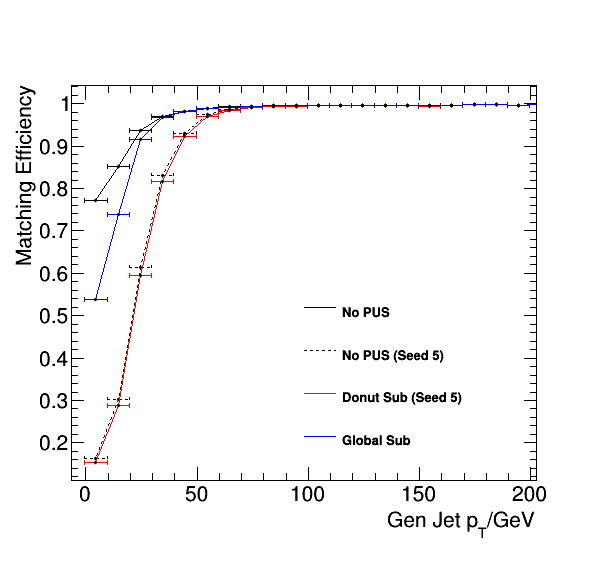
\includegraphics[width=7cm]{Figures/alljet}}
\hfill
\subfigure[4th jet\label{fig:label:jet4}]{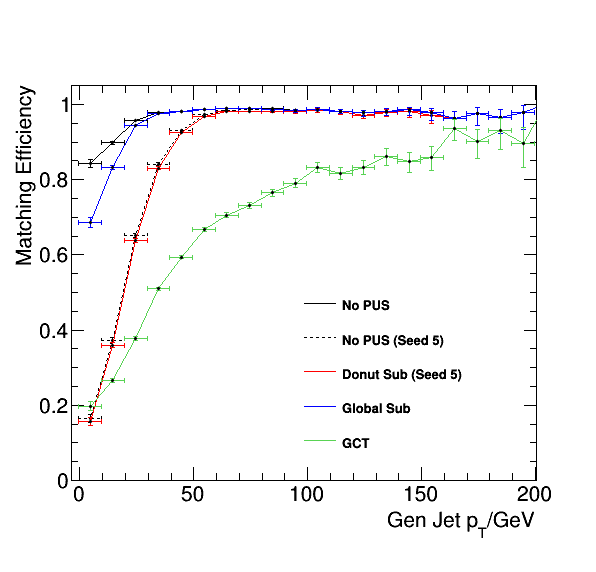
\includegraphics[width=7cm]{Figures/jet4}}
\hfill
\caption{Matching efficiencies for jets showing effect of seed and PUS at low energies. In \ref{fig:label:jet4} a comparison with the GCT is shown.}
\label{match}
\end{figure}
\subsection{Calibration}
The energy of the L1 jets must be calibrated using generator level quantities. The scheme for calibration is outlined in \cite{l1jet_calibration}. Essentially, using a QCD PU 40, 50ns sample, the resolution (defined as $p^{L1}_{T}/p^{gen}_{T}$) and $p^{L1}_{T}$ are plotted against $p^{gen}_{T}$ and fitted. The fits are then plotted against each other giving calibration factors as a function of $p^{L1}_{T}$. The calibration is carried out in bins of $\eta$ to account for the difference in performance of the detector. Where the matching efficiency is low it is not possible to fit and so the calibration has a lower bound on $p_T$. This was found to occur at $20GeV$. The calibration factors change depending on the PUS regime.    
\begin{figure}
\hfill
\subfigure[All jets\label{fig:label:alljet}]{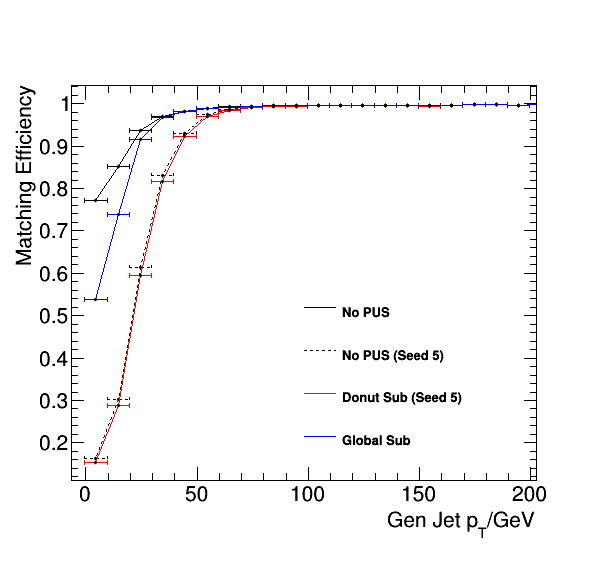
\includegraphics[width=7cm]{Figures/alljet}}
\hfill
\subfigure[4th jet\label{fig:label:jet4}]{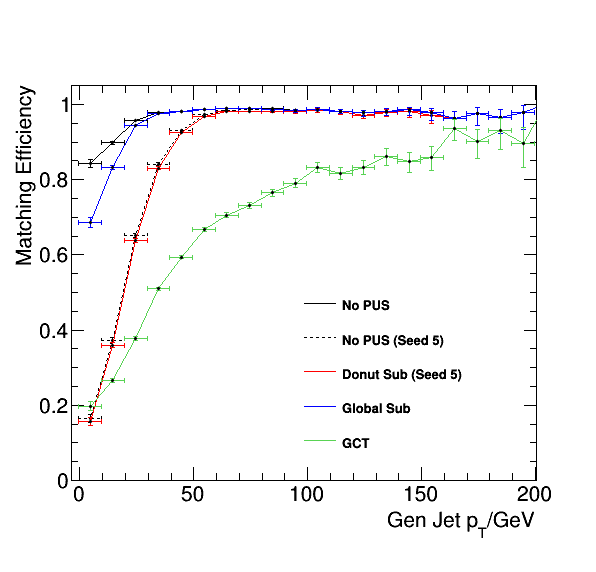
\includegraphics[width=7cm]{Figures/jet4}}
\hfill
\caption{Resolution before and after calibration. In \ref{fig:label:jet4} a comparison with the GCT is shown.}
\label{match}
\end{figure}
\section{PUS Testing}
\subsection{Reso}
In this section plots are shown for the highest $|\eta|$ bin as the detector perofrmance is expected to worsen with larger $|\eta|$ and so PUS will have the largest effect. The first test of any PUS scheme is the effect on the resolution. In an ideal post PUS scenario this will be flat as a function of NVTX. In figure \ref{fig:label:resolution1} this is plotted for a particular $p^{gen}_T$ and $\eta$ bin. It can be seen that the response flattens for both PUS regimes. This is summarised in \ref{fig:label:resolution2} where the gradient from the fit to the resolution plot is shown to reduce after PUS for a range of $p^{gen}_T bins$.  
\begin{figure}
\hfill
\subfigure[All jets\label{fig:label:resolution1}]{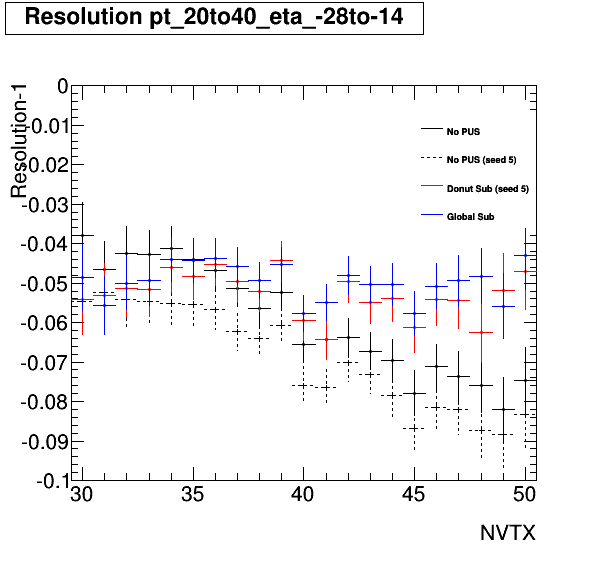
\includegraphics[width=7cm]{Figures/pt_20to40_eta_-28to-14}}
\hfill
\subfigure[All jets\label{fig:label:resolution2}]{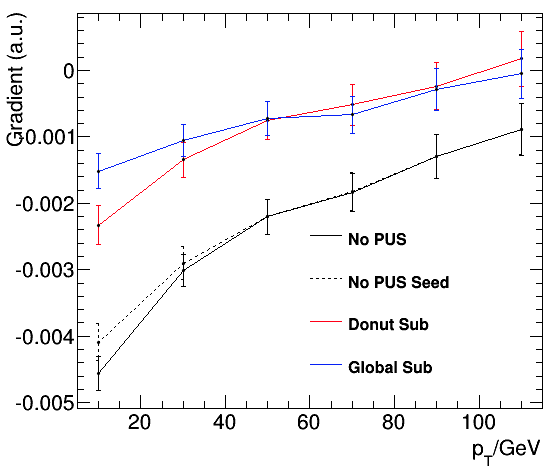
\includegraphics[width=7cm]{Figures/p1eta_14to28_calib_fits}}
\caption{In \ref{fig:label:resolution1} response versus NVTX is shown for a particular eta bin showing the response flattens after PUS. In \ref{fig:label:resolution2} the fit gradient for the response against NVTX for different $p_{T}$ bins is shown.}
\label{fig:label:resolution}
\end{figure}
\subsection{Rates}
The rate/efficiency is defined as the proportion of jets for signal/background passing a particular $p_{T}$ cut. For the trigger the key test is to see that the efficiency for signal may be maintained while reducing the background rate. Neutrino gun (PU40, 50ns) and ttbar (PU40, 50ns) samples were used as background and signal. In figure \ref{} the rate versus efficiency is plotted for the 4th jet. This shows PUS reducing the rate while maintaining efficiency. Performance compared to the GCT is shown to be greatly improved. This information is combined with the dependence on NVTX is shown in figure *. After PUS the rates are lower and the dependence on NVTX is reduced. 
\begin{figure}
\centering
    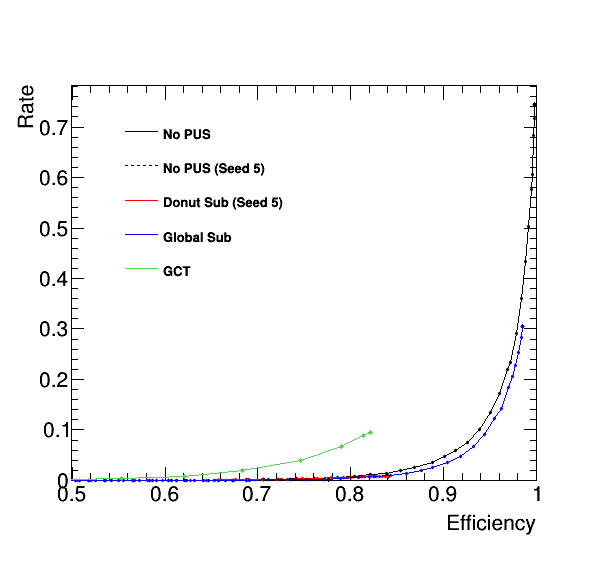
\includegraphics[width=0.8\textwidth]{Figures/rateeffjet4}
  \caption{Rate of a background (neutrino) sample against efficiency from a ttbar sample showing improvement after PUS.}
  \label{rateff}
\end{figure}
\begin{figure}
\hfill
\subfigure[All jets\label{fig:label:rateeff}]{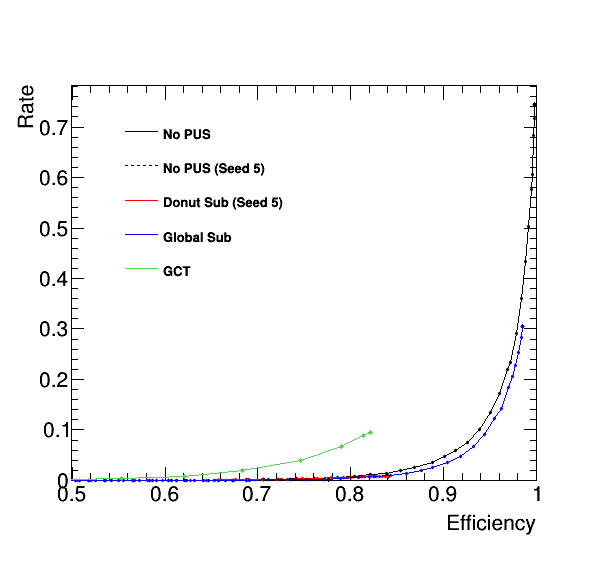
\includegraphics[width=7cm]{Figures/rateeffjet4}}
\hfill
\subfigure[All jets\label{fig:label:ratenvtx}]{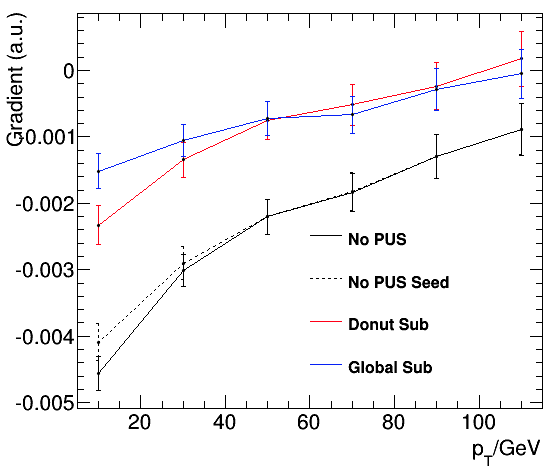
\includegraphics[width=7cm]{Figures/p1eta_14to28_calib_fits}}
\caption{In \ref{fig:label:resolution1} response versus NVTX is shown for a particular eta bin showing the response flattens after PUS. In \ref{fig:label:resolution2} the fit gradient for the response against NVTX for different $p_{T}$ bins is shown.}
\label{fig:label:resolution}
\end{figure}

 

%----------------------------------------------------------------------------------------
%	THESIS CONTENT - APPENDICES
%----------------------------------------------------------------------------------------

\addtocontents{toc}{\vspace{2em}} % Add a gap in the Contents, for aesthetics

\appendix % Cue to tell LaTeX that the following 'chapters' are Appendices

% Include the appendices of the thesis as separate files from the Appendices folder
% Uncomment the lines as you write the Appendices

%% Appendix A

\chapter{Coherent State Formalism} % Main appendix title

\label{AppendixA} % For referencing this appendix elsewhere, use \ref{AppendixA}

\lhead{Appendix A. \emph{Coherent States}} % This is for the header on each page - perhaps a shortened title
\section{Harmonic Oscillator}
First consider the harmonic oscillator in 1D quantum mechanics. The Hamiltonian is given by
\begin{equation}
{\bar H} = \frac{{\bar p}^2}{2m}+\frac{1}{2}m\omega^2{\bar q}^2
\end{equation}
where ${\bar p}$ and ${\bar q}$ are the momentum and position operators respectively and $\omega$ is the frequency of the oscillator. A state excited to level n is defined by
\begin{equation*}
\vert n \rangle = \frac{a^{\dagger}}{\sqrt{n!}}\vert 0 \rangle 
\end{equation*}
where $a$ is the annihilation operator. Consider now the state $\vert a \rangle$ defined by:
\begin{equation}
{\hat a} \vert a \rangle = a \vert a \rangle.
\end{equation}
Such a state is known as a coherent state. In the coordinate representation this may be written as
\begin{equation}
\label{harmcoh}
\langle q \vert a \rangle = N.exp(-\frac{1}{2}a^2-\frac{1}{2}\frac{\omega}{q^2}+\sqrt{2\omega}aq).
\end{equation}
The coherent state representation of $\vert n \rangle$ is given by
\begin{equation}
\psi_n(a^*) \equiv \langle a \vert n \rangle = \langle a \vert 0 \rangle \frac{(a^*)^n}{\sqrt{n!}}
\end{equation}
and to determine the constant $\langle a \vert 0 \rangle$ consider
\begin{equation}
1 = \sum_n \langle a \vert n \rangle \langle n \vert a \rangle =  {\vert \langle 0 \vert a \rangle \vert}^2 \mathrm{e}^{{\vert a \vert}^2}
\end{equation}
giving the normalisation
\begin{equation}
\langle a \vert 0 \rangle = \mathrm{e}^{-1/2{\vert a \vert}^2}.
\end{equation}
Normalising such that 
\begin{equation}
\psi_n(a^*) \equiv \langle a \vert n \rangle = \frac{(a^*)^n}{\sqrt{n!}},
\end{equation}
the completeness relation is then written as
\begin{equation}
\label{comp}
\int \frac{\mathrm{d}^2a}{\pi} \mathrm{e}^{-{\vert a \vert}^2} \vert a \rangle \langle a \vert = 1
\end{equation}
where
\begin{equation}
a = r\mathrm{e}^{i\theta} \rightarrow \mathrm{d}^2a = rdrd\theta 
\end{equation}
and the scalar product between states is written
\begin{equation}
\label{scalp}
\langle \psi_n \vert \psi_m \rangle = \int \mathrm{e}^{-{\vert a \vert}^2} \frac{\mathrm{d}^2a}{\pi} [\psi_n(a^*)]^*\psi_m(a^*).
\end{equation}
Operators are defined by their kernel $A(b^*,a) \equiv \langle b \vert {\hat A} \vert a \rangle $ and act as
\begin{equation}
\label{kern}
({\hat A} \psi)(b^*) = \int \mathrm{e}^{-{\vert a \vert}^2} \frac{\mathrm{d}^2a}{\pi} A(b^*,a)\psi(a^*).
\end{equation}
Finally the overlap between two coherent states is given by:
\begin{equation}
\label{overlap}
\langle a \vert b \rangle = \sum_n \langle a \vert n \rangle \langle n \vert b \rangle = \sum_n \frac{{a^*b}^n}{n!} = \mathrm{e}^{a^*b}.
\end{equation}
\section{Scalar Field Theory}
These results may be translated to field theory where the states are eigenstates of the annihilation operator of momentum $k$, ${\hat a_k}$ 
\begin{equation}
{\hat a_k}\vert \{a_k\}\rangle = a_k \vert \{a_k\}\rangle \forall k
\end{equation}
The starting point for Chapter \ref{Chapter3} is the generalisation of \ref{harmcoh} to scalar field theory which gives
\begin{equation}
\langle \phi \vert \{a_k\}\rangle = N.exp\left[-\frac{1}{2} \int \mathrm{d} k a_k a_{-k} -\frac{1}{2} \int \mathrm{d} k \omega_k {\tilde \phi}(k){\tilde \phi}(-k)+\int \mathrm{d}k \sqrt{2\omega_k} a_k {\tilde \phi}(k)\right]
\end{equation}
where 
\begin{equation}
\frac{1}{(2\pi)^{3/2}}\int \mathrm{d}x e^{ik.x}\phi(x) \equiv {\tilde \phi}(k)
\end{equation}
is the spatial Fourier transform of $/phi(x)$. Equations \ref{comp}, \ref{scalp} and \ref{kern} are generalised similarly.
%% Appendix Template

\chapter{Saddle Point Method} % Main appendix title

\label{AppendixB} % Change X to a consecutive letter; for referencing this appendix elsewhere, use \ref{AppendixX}

\lhead{Appendix B. \emph{Saddle Points}} % Change X to a consecutive letter; this is for the header on each page - perhaps a shortened title

This derivation follows \citep{MOMP}. Consider an integral of the form
\begin{equation}
I(N) = \int_a^b\mathrm{d}z g(z)\mathrm{e}^{Nf(z)} \; \; N \gg 0
\end{equation}
where $f(z)$ is a complex analytic function and $N$ is a real number. Define $f(z) = u +iv$, the integral will be dominated by values of $u$ near its maximum. On the other hand if $v$ is not stationary then the oscillating contributions will cancel. This implies the largest contribution will be for $f'(z)=0$. This must be a saddle point of $f(z)$. In the case of several saddle points the integral is dominated by the highest. Assuming this is at $z_0$ by Cauchy's integral theorem the contour may be deformed such that it goes through that point. Near $z_0$ $g(z) \simeq  g(z_0)$ and $f(z)$ can be written as 
\begin{equation}
f(z) \simeq f(z_0)+ \frac{1}{2} f''(z_0)(z-z_0).
\end{equation}
The integral then becomes
\begin{equation}
I(N) \simeq g(z_0)\mathrm{e}^{Nf(z_0)} \oint_C\mathrm{d}z exp\left[\frac{1}{2}Nf''(z_0)(z-z_0)^2\right].
\end{equation}
Using a change of variables as
 \begin{equation*}
z-z_0 = r\mathrm{e}^{i\phi} \;\; f''(z_0) = \vert f''(z_0) \vert \mathrm{e}^{i\theta}
\end{equation*}
The choice of $\phi$ will not affect the result as this only controls the approach angle of the contour to the saddle point. By choosing it as $\phi = (\pi - \theta)/2$ the integral simplifies to
\begin{equation}
I(N) \simeq g(z_0)\mathrm{e}^{Nf(z_0)}\mathrm{i\phi} \int\mathrm{d}r exp\left[-\frac{1}{2}N\vert f''(z_0)\ vert r^2\right]
\end{equation}
This is now just a Gaussian integral and the result is
\begin{equation}
I(N) \simeq g(z_0)\mathrm{e}^{Nf(z_0)}\mathrm{i\phi} \frac{2\pi}{\vert Nf''(z_0)\vert}^2.
\end{equation}
This is the saddle point approximation to the integral. It is also known as the method of steepest descent. This is because this choice of $\phi$ corresponds to a path of steepest descent from the saddle point.

%% Appendix C

\chapter{Symmetric Double Well} % Main appendix title

\label{AppendixC} % For referencing this appendix elsewhere, use \ref{AppendixA}

\lhead{Appendix C. \emph{Symmetric Double Well}} % This is for the header on each page - perhaps a shortened title
\section{Symmetric Double Well}
\begin{figure}[htbp]
	\centering
		\includegraphics[width=0.8\textwidth]{./Figures/symmwell}
	\caption[Symmetric Double Well]{The symmetric double well has a degeneracy in the minima, complicating the solution}
	\label{fig:symmwell}
\end{figure}
The derivation for a symmetric double well follows exactly that for the case of false minimum decay up to \ref{sumall}. Consider figure \ref{fig:symmwell}. By symmetry it is possible to start and end an instanton path in either $x=\pm a$. For false vacuum decay there is no degeneracy between the minima and so an instanton path had to start and end at $x=0$. Now, however, this is no longer the case and so an instanton is taken to refer to a path which starts at $x=-a$ and ends at $x=+a$ while an anti-instanton refers to the opposite path. By symmetry both give the same contribution and will be referred to as bounces (K is implicitly redefined to account for this).  However, there will be a difference in the case which ends at the opposite minimum to that which does not as $\tau_0\rightarrow\infty$. In the first case there will be an odd number of bounces and in the second an even number. Therefore the sum for each case will be over odd and even numbers of pseudo particles respectively.
\begin{equation}
\langle \pm a \vert \mathrm{e}^{-H\tau_0} \vert a \rangle = \sum_{n even/n odd}^{\infty}  \left(\frac{\omega}{\pi}\right)^{1/2} \mathrm{e}^{-\omega \tau_0/2}\frac{\left(K\mathrm{e}^{-S_0}\right)}{n!}=\left(\frac{\omega}{\pi}\right)^{1/2}\mathrm{e}^{-\omega\tau_0/2}\frac{1}{2}\left[exp(K\mathrm{e}^{-S_0}T) \pm exp(-K\mathrm{e}^{-S_0}T)\right].
\end{equation}
Therefore there are now two eigenstates with energies
\begin{equation}
\label{shift}
E_{\pm} = \frac{1}{2}\omega \pm K \mathrm{e}^{-S_0}
\end{equation}
Denoting these eigenstates by $\vert + \rangle$ and $\vert - \rangle$ the expectation values may also be read
\begin{equation}
{\vert \langle + \vert \pm a \rangle \vert}^2 = {\vert \langle - \vert \pm a \rangle \vert}^2 = - \langle a \vert - \rangle \langle - \vert -a \rangle = -\langle a \vert + \rangle \langle + \vert -a \rangle =\frac{1}{2}\left(\frac{\omega}{\pi}\right)^{1/2}
\end{equation}
and so there is not a degeneracy in the particle position but instead it can exist in either well with the effect of tunnelling ``smearing" the ground states. The lowest energy state will be that with an even superposition of the wavefunctions in each well while the higher energy corresponds to an odd superposition.  The shift of the energy in \ref{shift} is actually much smaller than neglected terms due to the exponential suppression. It is included, however, as this is the highest order term in the energy difference between these two states. It is shown in \citep{instln} that this gives the correct result for the potential $V = \lambda(x^2-\eta^2)^2$. 

\addtocontents{toc}{\vspace{2em}} % Add a gap in the Contents, for aesthetics

\backmatter

%----------------------------------------------------------------------------------------
%	BIBLIOGRAPHY
%----------------------------------------------------------------------------------------

\label{Bibliography}

\lhead{\emph{Bibliography}} % Change the page header to say "Bibliography"

\bibliographystyle{unsrtnat} % Use the "unsrtnat" BibTeX style for formatting the Bibliography

\bibliography{Bibliography} % The references (bibliography) information are stored in the file named "Bibliography.bib"

\end{document}  
